% !TeX program = pdflatex
% !TeX root = Thesis.tex

\documentclass[english]{saartex}
% This file contains "basic" options.
% For more advanced ones, you might have
% to edit Thesis.cls

% Base Font Size
%   All other font sizes (for headings etc.) are adjusted accordingly

\KOMAoptions{fontsize=12pt}

% Depth of table of contents
%   0 displays only parts and chapters, 1 displays parts, chapters and sections, etc.

\setcounter{tocdepth}{1}

% Use the specific citation style
%   The value after "style=" specifies the style
%   common values include "numeric", "alphabetic", "authoryear"
%   for a reference see http://mirrors.ctan.org/macros/latex/contrib/biblatex/doc/biblatex.pdf#subsection.3.3
\usepackage[style=numeric,sorting=none]{biblatex}
\usepackage{caption}

% Thesis-specific table and math helpers. Keep this list small so that it
% remains compatible with the SaarTex class and pdfLaTeX.
\usepackage{booktabs}
\usepackage{tabularx}
\usepackage{bm}
\usepackage{xspace}
\usepackage{todonotes}
\usepackage{bbm}

% Put figures in the Figures/ directory and include them by file name, e.g.
% \includegraphics[width=\linewidth]{my-figure}
\graphicspath{{Figures/}}

% Print the whole bibliography?
%   By default, LaTeX prints just those bibliography items that have been cited.
%   If you want to print the whole bibliography, uncomment the following line
%   
%   \nocite{*} 

\def\sign{{\text{sign}}}
\addbibresource{Literature.bib}

\title{Benchmarking Robustness of Self-Supervised Learning Across Diverse Downstream Tasks}
\author{Antoni Kowalczuk}
\subject{Master Thesis}
\place{Saarbrücken}
\advisor{Dr. Adam Dziedzic}
\professor{Prof. Dr. Andreas Zeller}
\date{\today}

\DeclareMathOperator*{\argmax}{arg\,max}
\DeclareMathOperator*{\argmin}{arg\,min}
\newcommand{\EmbedAttack}{\textsl{EmbedAttack}\xspace}
\newcommand{\PGD}{\textsl{PGD}\xspace}
\newcommand{\SegPGD}{\textsl{SegPGD}\xspace}
\newcommand{\DepthPGD}{\textsl{DepthPGD}\xspace}
\newcommand{\DeACL}{\textnormal{\textsc{DeACL}}\xspace}
\newcommand{\DINO}{\textnormal{\textsc{DINO}}\xspace}
\newcommand{\DINOv}{\textnormal{\textsc{DINOv2}}\xspace}
\newcommand{\eg}{\textit{e.g.,}\@\xspace}
\newcommand{\ie}{\textit{i.e.,}\@\xspace}

\begin{document}

\hypersetup{plainpages=false,pageanchor=false}
\maketitle
\frontmatter
\hypersetup{pageanchor=true}

\chapter*{Abstract}
\addcontentsline{toc}{chapter}{Abstract}
\markboth{Abstract}{Abstract}

Self-supervised (SSL) image encoders find broad applications across many domains. They output rich representations---high-dimensional continuous vectors---of the input images. These representations are useful for a plethora of downstream tasks,~\eg classification, image segmentation, or object detection. There, a simple linear probing achieves very high performance, despite the SSL encoders never being trained directly to perform well on these tasks.

Their success brought ubiquitus use-cases, from medical image analysis, to self-driving cars. With their presence in such critical areas, there come inevitable harms, when these models fail. One of the (many) failure modes are so-called adversarial images. These images are crafted by adding imperceptible perturbations to the benign images, where the perturbations are optimized to cause misprediction, while staying as small as possible, to avoid detection. 

While adversarial images have been extensively studied for classifiers, which output per-class probabilities, the literature for SSL encoders lags behind. The main reason for that is the representations they output reside in highly abstract, high-dimensional space, and there is no clear optimization direction for the perturbations. In contrast, for classifiers the goal is simple: flip the predicted class from the correct to an incorrect one. Moreover, the final use-case of each representation is unknown, which further obfuscates the optimization objective.

In this work, I close that gap, proposing \EmbedAttack, a downstream-task agnostic adversarial attack for SSL. With \EmbedAttack I craft adversarial images, which cause severe misclassification downstream, regardless of the task. Across multiple datasets, \EmbedAttack shows TODO SOME NUMBERS, highlighting its effectiveness. Compared to downstream-specific attacks like \PGD and \SegPGD, \EmbedAttack achieves comparable, yet slightly worse performance HERE MORE NUMBERS, since it does not exploit the knowledge of the downstream task other attacks optimize against.

My work shows that 1) universal, dataset- and task-agnostic adversarial attacks ągainst SSL encoders are possible; 2) performance of \EmbedAttack is strong enough to cause significant prediction errors on real SSL encoders.

\tableofcontents
\ifgerman{\chapter*{Eidesstattliche Erklärung}

\pagestyle{plain}

Ich erkläre eidesstattlich, dass ich diese Arbeit selbstständig verfasst und fremde Quellen und Gedanken kenntlich gemacht habe. Sie wurde keiner Prüfungsbehörde vorgelegt oder veröffentlicht. Mir sind rechtliche Folgen unwahrer Angaben bewusst.

\vfill

\vspace*{\baselineskip}
\noindent \begin{minipage}{\textwidth}
	\noindent \begin{minipage}{0.49\textwidth}
		\begin{flushleft}
			\usenonemptytitleelement{place}, \rule{3cm}{0.5pt}
		\end{flushleft}
	\end{minipage} \hfill
	\begin{minipage}{0.49\textwidth}
		\begin{flushright}
			\rule{4cm}{0.5pt}
		\end{flushright}
	\end{minipage}
\end{minipage}

\newpage
}
\ifenglish{\chapter*{Sworn declaration}

\pagestyle{plain}

I declare under oath that I prepared this thesis independently, used only the stated sources and resources, and marked all literal or corresponding borrowings. This thesis has not previously been submitted to any examination board in the same or similar form.

\vfill

\vspace*{\baselineskip}
\noindent \begin{minipage}{\textwidth}
	\noindent \begin{minipage}{0.49\textwidth}
		\begin{flushleft}
			\usenonemptytitleelement{place}, \rule{3cm}{0.5pt}
		\end{flushleft}
	\end{minipage} \hfill
	\begin{minipage}{0.49\textwidth}
		\begin{flushright}
			\rule{4cm}{0.5pt}
		\end{flushright}
	\end{minipage}
\end{minipage}

\newpage
}

\cleardoublepage
\mainmatter

\chapter{Introduction}\label{chap:introduction}

In this section I introduce the main object of my study: image encoders trained under self-supervised learning (SSL) TODO CITE paradigm. After providing an overview of what SSL is and why it was invented, I pivot to the second topic: adversarial images TODO CITE. Finally, I pair both topics, highligh the research gap my work addresses, and summarize the contributions of this thesis.

\section{Computer Vision}

% 3 pages more or less here

The main objective of computer vision is to give sight to the computers. Our cameras already provide a lot of raw data, comprising of millions of 8bit numbers per image. The computer should "make sense" of this data,~\ie understand the image's contents, semantics, structure, etc. The understanding should be at least partially similar to how we, humans, see and reason visually. 

One of the ways to give an actual understanding came from an advent of machine learning (ML), where neural networks (NNs), optimized to minimize prediction error, achieved reasonable classification accuracy on ImageNet-1k TODO ADD CITATIONS. These models use sizeable sets of data, comprising of images, labelled manually by human workers into classes.

While their success is impressive, with current performance on ImageNet-1k benchmark surpassing human-eye-ball-based "classifiers", they rely heavily on manual labor for data collection, processing, filtering, and finally: labelling. ImageNet-1k, while truly ahead of its time, comprises of only 1M image+label pairs. The Internet offers orders-of-magnitude more data, albeit unlabeled, waiting to be harnessed.

\section{Self-Supervised Learning and Image Encoders}

One of the approaches to use this data productively, studied in this work, is self-supervised learning (SSL). There, the NNs are optimized towards a different objective than predicting the correct label, due to the lack of one. Instead, they output high-dimensional vectors, referred to as representations or embeddings throughout this thesis. Representations are meant to encode the rich contents of an image (usually consisting of milliions of pixels) into significantly sparser, continuous point in an embedding space. 

These representations have many use-cases. One can train a simple logistic regression model, which predicts an image's class based on the SSL model's embeddings. Contrary to big and expensive to train networks, such an approach is cheap, and oftentimes beats NNs trained from scratch just to solve a specific task. Similarly, recent SSL encoders like DINO (TODO CITE) enable per-pixel predictions, for example segmentation or depth estimation. 

While embeddings are useful, now it's the time to discuss how they are obtained. Since random vectors are far from useful, the SSL encoders have to somehow derive how to craft a rich and expressive embeddings, using unlabeled data. The dominant approach here is to craft multiple "views" of an image,~\ie semantics-preserving augmentations like blurring or cropping. The NNs are trained to output identical representations for all views for the same image, and output different representations for views of two different images.

Training frameworks of SSL encoders vary. SimCLR HERE HOW IT TRAINS. SimSiam operates on siamese networks TODO CITE and stop-gradient operations to prevent collapse. DINO employs a self-distillation framework, where the teacher model is passed a "strong" view of the image, while the student sees a "weak", more noisy view of the same image. DINO is also the first framework to successfully use Vision Transformers (ViTs) TODO CITE for SSL. Thanks to ViT's attention mechanism TODO CITE it enables per-pixel predictions,~\eg segmentation.

\section{Adversarial Images}

Since SSL encoders are so powerful, they find many applications,~\eg in self-driving cars, or medical image processing CITE. These posits them as a crucial part in critical systems, and their failure can thus have severe negative consequences. 

While there are many modes of failure an ML system can have, this work focuses on one: adversarial images (also referred to as adversarial examples throughout this work). Adversarial images are crafted explicitly to cause misprediction of a victim ML model. It uses a clean, benign image, and subtly alters it to,~\eg flip the class prediction from correct to incorrect. The perturbation added to the original image is oftentimes simply invisible for a human eye, while the NN is consistently fooled. This makes the detection, counteraction, and monitoring of such a threat extremely difficult. 

Adversarial examples rely on gradient flow from the output of the NN back to the input image, hence they often require white-box access to the attacked model. Usually, they are created by crafting as small perturbation as possible that achieves the goal of misprediction,~\eg misclassification, using simple gradient-based optimization like PGD or FGSM TODO CITE. Adversarial examples are uniformly present, almost every NN is vulnerable to them, and after more than a decade of research, the solution is far from known. TODO ADD CITATIONS EVERYWHERE

\section{This work: SSL and Adversarial Examples}

Literature on adversarial images for classification is extensive, while this topic is less explored for SSL models. 
The reasons for that are as follows. 

First, the optimization objective for adversarial images against SSL models is non-obvious. These predict vectors that reside in complex high-dimensional space, and it is not clear what goal should an adversarial image achieve there, and what to optimize for. 

Second, the actual success of the attack is unknown, unless the adversary (attacker) explicitly knows what would this specific image's embedding be used for. This complicates the evaluation severely, as the attack success should be evaluated across a plethora of downstream tasks and datasets, especially since modern SSL models enable more than simple classification. 

Finally, the attack should be \textit{downstream-task-agnostic}, meaning it should cause misclassification for any downstream linear probe. Current literature focuses only on \textit{task-specific} attacks TODO CITE, which motivates work on a universal attack.

My contributions are as follows.
\begin{itemize}
    \item I introduce \EmbedAttack, a \textit{downstream task- and dataset-agnostic} adversarial attack against SSL image encoders.
    \item I evaluate \EmbedAttack against existing \textit{task- and dataset-specific} \PGD and \SegPGD for classification and semantic segmentation of images.
    \item I show that \EmbedAttack is reliable and universal, across XXX datasets, XXX tasks, and XXX SSL encoders, performing similarly to stronger, specific attacks.
\end{itemize}


















% Foundation vision models are valuable because they separate expensive representation learning from downstream use. A self-supervised encoder can be trained once on large image collections and later paired with small adaptors for classification, semantic segmentation, depth estimation, or retrieval. This reuse is the motivation behind modern self-supervised learning (SSL): unlabeled data supplies the pre-training signal, while task labels are needed only after the representation has been learned \parencite{chen2020simple,simsiam,caron2021dino,mae,balestriero2023cookbook}.

% The same reuse makes robustness evaluation difficult. If an encoder is deployed through many downstream heads, then a robustness claim about only one head is incomplete. Prior robust SSL work commonly evaluates a frozen encoder with a linear classifier and reports robust classification accuracy \parencite{NaseerPurifier2020CVPR,kim2020adversarial,jiang2020robust,fan2021does,zhang2022decoupled,luo2023rethinking}. Linear evaluation is useful, but it is only one interface. Dense tasks such as semantic segmentation and depth estimation expose pixel-wise losses and spatial tokens. An attacker that optimizes those outputs may find failures that a representation-level or classification-only evaluation does not reveal.

% This thesis rewrites the project around the resources provided in the repository. The central material is the manuscript and workshop work on evaluating adversarial robustness of SSL encoders across downstream tasks, together with the poster, figures, and thesis template. The resulting thesis focuses on one question:

% \begin{quote}
% \emph{Does adversarial robustness of a self-supervised vision encoder transfer across the downstream tasks for which foundation encoders are reused?}
% \end{quote}

% The empirical answer is negative in the evaluated setting. Standard \DINO and \DINOv encoders are strong clean representations, but are highly vulnerable to small $\ell_\infty$ perturbations. \DeACL, a state-of-the-art decoupled adversarial fine-tuning method, improves robustness against the representation attack used during robustification, but it does not reliably protect downstream task losses.

% \section{Motivation}

% Self-supervised encoders are no longer evaluated only as feature extractors for image classification. \DINO shows that self-distilled ViTs learn visual features useful for downstream tasks \parencite{caron2021dino}. \DINOv scales this idea and reports strong performance on both sparse and dense visual tasks \parencite{oquab2024dinov2}. If such encoders are foundation models, their robustness should be tested at the same breadth as their clean utility.

% Adversarial robustness is an interface-specific property. A perturbation can be generated to change an encoder embedding, a class prediction, a segmentation mask, or a depth map. These objectives are related but not identical. Representation stability may help downstream tasks, but it does not guarantee that every downstream loss is stable. Conversely, a segmentation attack can exploit pixel-wise errors that do not dominate a global representation metric.

% \section{Research Questions}

% The thesis investigates four research questions.

% \begin{enumerate}[wide]
%     \item How vulnerable are standard self-supervised vision encoders under embedding-level and downstream-task adversarial attacks?
%     \item Does \DeACL robust fine-tuning improve clean or robust performance across classification, segmentation, and depth estimation?
%     \item Are representation-level attacks sufficient proxies for task-specific attacks?
%     \item What evaluation protocol is appropriate for robustness claims about reusable foundation encoders?
% \end{enumerate}

% \section{Contributions}

% The thesis makes three contributions.

% \textbf{First,} it organizes adversarial robustness for SSL encoders around two attack interfaces: \EmbedAttack in encoder space and downstream \PGD-style attacks against task losses. This distinction follows the encoder/adaptor deployment pattern.

% \textbf{Second,} it gives a unified thesis presentation of the supplied robustness resources. The evaluation covers classification on CIFAR10, CIFAR100, and STL10; semantic segmentation on ADE20K, Cityscapes, and PASCAL VOC 2012; and monocular depth estimation on NYU-Depth v2.

% \textbf{Third,} it derives the main lesson for foundation-model evaluation: clean transfer and representation robustness are not enough. A reusable encoder should be reported with clean and adversarial metrics for every relevant downstream task and attack surface.

% \section{Structure}

% \Cref{chap:background} introduces SSL, \DINO-family encoders, downstream adaptation, adversarial attacks, and robust SSL. \Cref{chap:ssl-method} defines the experimental setting, attacks, and \DeACL defense. \Cref{chap:evaluation} reports results. \Cref{chap:discussion} concludes the thesis after the extended-details chapter records related work, hyperparameters, and loss details.

\chapter{Background}
\label{chap:background}

% 5 pages imo

In this chapter I introduce the literature background for the thesis. I begin with a comprehensive overview of existing and examined SSL training frameworks, focusing on the architectures, training, evaluation, and downstream tasks. Then, I provide a breakdown on adversarial examples, explaining the theory behind them, their universality, current attacks, and pair them with current SSL paradigm.

\section{SSL Vision Encoders}

Contrary to classification task, where the goal is to predict a correct class $c\in\{1, 2,...,K\}$ from possible $K$ classees, based on the image $x\in\mathbb{R}^{C\times H\times W}$, the goal of SSL encoders is more general. Classifiers learn based on labeled data $(x, c)$, under supervised learning paradigm,~\ie the correct prediction is well known, and the sole training objective is to teach the NN to output a specific (correct) class $c$ for each image $x$.

SSL abandons the luxury of labeled data. Intuitively, most of the data one can obtain via Internet-scale scraping is unlabeled, and the labeling requires costly human labor. Without labels, SSL posits an alternative training objective,~\ie representation learning. Representations $z\in\mathbb{R}^d$ are understood as high-dimensional ($d$ denotes number of dimensions), continuous vectors. After training, the SSL model $f_\theta: \mathbb{R}^{C\times H\times W}\rightarrow\mathbb{R}^d$ (with parameters $\theta$) should output rich and expressive representation $z$ of any image $x$, enabling further downstream use of the representations.

\subsection{Training Paradigms}

Notably, what exactly is a "rich and expressive representation $z$ of any image $x$, enabling further downstream use of the representations" is not well-grounded in theory. Moreover, one cannot compute gradient of such an objective. 

More precise view of the above goal is: representations $z_1$, $z_2$ of two \textit{similar} images $x_1$, $x_2$ should be \textit{closer} than representations $z_1$, $z_3$ of two \textit{dissimilar} images $x_1$, $x_3$. Intuitively, an image of a dog should have a representation that lies close to other images of dogs in the embedding space, and should have a representation that lies far from images depicting circuit boards. 

\subsection{Similar Images and SSL}
\label{sec:similar_imgs_ssl}

Defining "similarity" of images is tricky, especially since images can be similar in many ways. The similarity may be structural, compositional, semantic, stylistic, etc. To avoid ambiguities and human-based biases, the default approach is to augment \textit{the same} image multiple times, producing multiple "views". These views are (likely) similar to each other, and the similarity is as broad as imaginable. 

Representations' "closeness" is easier to precisely formulate. Since embeddings are continuous vectors, the natural approach is to use an abstract \textit{distance} function $\text{dist}: \mathbb{R}^d\times\mathbb{R}^d\rightarrow\mathbb{R}$, for example L2 distance or cosine similarity. 

Effectively, given a dataset of $N$ unlabeled images $D=\{x_i\},i=1,...,N$ the SSL training objective utilizing multiple views of the same image is as follows:

\begin{equation}
    \label{eq:loss_ssl_sim}
    \theta^*=\underset{\theta}{\argmin}
        \mathbb{E}_{x\sim D,\mathcal{A}_i\sim{\mathbb{A}},\mathcal{A}_j\sim\mathbb{A}}
        \left[
        \text{dist}(\mathcal{A}_i(x),\mathcal{A}_j(x))
        \right]\text{,}
\end{equation}
where $\mathbb{A}=\{\mathcal{A}_1,\mathcal{A}_2,...\}$ is a set of augmentations $\mathcal{A}_i: \mathbb{R}^{C\times H\times W} \rightarrow \mathbb{R}^{C\times H\times W}$.

\subsection{The Great Collapse}

Unfortunately,~\cref{eq:loss_ssl_sim} has a fatal flaw: its minimizer is a network $f_\theta^*: \mathbb{R}^{C\times H\times W}->[0]^d$. To address that HERE SIMSIAM AND DINO ONCE I HAVE INTERNET TO WRITE IT AS GOOD AS IT GETS.

\subsection{Dissimilar Images and Contrastive Learning}

While \textit{similar} images' embeddings should stay close, it is also important that \textit{dissimilar} images' embeddings stay far from each other. Analogously to~\cref{sec:similar_imgs_ssl}, it is not clear what does exactly mean that two images are dissimilar. 

The trivial solution is to assume that two different images are dissimilar from the definition. Contrastive Learning assumes exactly that, with the InfoNCE training loss defined as:

\begin{equation}
    \label{eq:infonce}
    \text{InfoNCE}=
\end{equation}

Intuitively, this training objective forces the NN to "push away" the representations of all alterantive images from the original positive image. Such a paradigm has been widely adopted HERE MORE ABOUT SIMCLR, AND MAYBE ABOUT CLIP.

ALSO ABOUT THE TRAINING DATA, IMAGENET, HOW MANY EPOCHS, THAT A LOT OF STUFF IS STANDARDIZED ETC.

\subsection{Evaluating SSL Image Encoders}

The generality of the SSL training task (\cref{eq:loss_ssl_sim,eq:infonce}) comes at a cost. One can not simply look at the produced embeddings $z$ and assess their quality, since their dimension $d$ is often too high (above 100, sometimes even 1000) to allow for meaningful analysis, yet alone a universal quality metric.

Instead, researchers focus on measuring how useful the embeddings are to help solve well-defined tasks, like classification or semantic segmentation. For classification, the dominant approach is to select a downstream dataset $D_T=\{(x_i,c_i)\}, i=1,...,N_T$ of $N_T$ labeled images, and based on the representations from trained $f_\theta$, fit a simple linear model $l_\mathbf{w}: \mathbb{R}^d \rightarrow \{1,...,K\}$ minimizing cross-entropy loss $\text{CELoss}=-\log(1-p_i)$, where $p_i$ is the probability of i-th class returned by $l_\mathbf{w}$. The final encoder+linear model classification stack is defined as

\begin{equation}
    (l_\mathbf{w}\circ f_\theta): \mathbb{R}^{C\times H\times W} \rightarrow \{1,...,K\}\text{,}
\end{equation}
and its downstream task performance is evaluated as accuracy on the validation set of the training data $D_T$. The established approach is to perform a single training epoch on the downstream data.

TODO HERE ABOUT segmentation


\section{Adversarial Examples}

While most of the field focused on making the models better and more general, TODO CITET indentified a grave vulnerability of almost every neural network that exists. With some assumptions (introduced later) and little effort, any NN can be forced to output a wrong prediction with high consistency. What is even worse, such an adversarial input to the NN can be made indistinguishable from a real, benign input, and can evade detection. Changing a few pixel values by extremely small values (for example by at most 8/255 of the full pixel range) is enough to reliably fool a vast majority of image-based NNs, regardless of their training data, training objective, architecture, hyperparameters, preprocessing, and so on.

TODO CITIT AGAIN dubbed their discovery as "adversarial examples". More precisely, an adversarial example $x_{adv}=x+\delta$ is a benign sample $x$ (here: image) and its perturbation $\delta$, crafted explicitly to cause misprediction of a victim model $f_V$. To limit the difference between clean and adversarial image, $\delta$ is oftentimes constrained to be $\left\|\delta\right\|_p<\epsilon$, where $p\in\{0,1,2,\infty\}$. To ensure imperceptibility, $\epsilon$ is usually very small,~\eg $8/255$ for $L_\infty$ norm, meaning each pixel of the image is changed by at most $8/255$ (assuming pixel values are in $[0,1]$).

Another important element of adversarial examples is the optimization procedure to obtain $\delta$. Given an adversarial objective, 

Here more about the theory that the errors will accumulate etc

PGD here

SegPGD here































% This chapter summarizes the technical background needed for the robustness evaluation: reusable vision encoders, SSL objectives, downstream tasks, adversarial attacks, and robust SSL defenses.

% \section{Foundation Vision Encoders}

% Foundation models are trained at scale and then adapted to tasks that are not fixed during pre-training \parencite{bommasani2021opportunities}. In vision, the foundation component is often an encoder $f_\theta$ that maps an image $x$ to a representation $z=f_\theta(x)$. A downstream adaptor $h_\phi$ maps $z$ to the task output. For classification the output is a class label; for segmentation it is a pixel-label map; for depth estimation it is a dense continuous depth map.

% Vision Transformers (ViTs) are a natural backbone for this setting \parencite{dosovitskiy2020image}. An image is divided into patches, each patch is embedded as a token, and transformer blocks process the token sequence. Classification can use a class token or pooled token, while dense tasks use patch tokens and upsampling heads. The architecture therefore exposes both global and spatial representations.

% \section{Self-Supervised Learning}

% SSL learns representations without manual labels. A common formulation samples two augmentations $x_1$ and $x_2$ of the same image and trains the encoder so that their representations agree \parencite{chen2020simple,balestriero2023cookbook}. SimCLR uses a contrastive objective that attracts positive pairs and repels negatives \parencite{chen2020simple}. SimSiam removes explicit negatives and uses a stop-gradient Siamese structure \parencite{simsiam}.

% \DINO uses self-distillation \parencite{caron2021dino}. A student network predicts the output distribution of a teacher network on a different augmented view; the teacher is updated as an exponential moving average of the student. Centering and sharpening avoid collapse. \DINO features are especially relevant because they transfer well to ViT downstream tasks.

% \DINOv extends this line at larger scale and with stronger training recipes \parencite{oquab2024dinov2}. It is important for this thesis because its representations are explicitly used for diverse tasks, including dense prediction. A robustness evaluation that only tests linear classification is therefore narrower than the claimed deployment value.

% \section{Downstream Tasks}

% \textbf{Linear classification} is the standard SSL evaluation protocol. The encoder is frozen and a linear classifier is trained on top of its representation \parencite{chen2020simple,simsiam}. Accuracy measures how linearly separable the learned representation is.

% \textbf{Semantic segmentation} assigns a class to every pixel. Fully convolutional networks established the dense prediction setting \parencite{long2017segmentation}, and UPerNet introduced unified multi-scale parsing for scene understanding \parencite{xiao2018unified}. For frozen ViTs, segmentation heads consume patch tokens, upsample logits, and optimize pixel-wise cross-entropy. Performance is reported as mean intersection-over-union (mIoU).

% \textbf{Monocular depth estimation} predicts a depth value from a single RGB image. It is dense like segmentation, but the output is continuous and geometric. Depth training often combines pixel-wise scale-invariant errors with gradient or smoothness terms \parencite{godard2019depthestimation,MegaDepthLi18,AdaBins}. This thesis reports root mean squared error (RMSE), where lower is better.

% \section{Adversarial Robustness}

% Adversarial examples are small perturbations that cause incorrect or degraded predictions \parencite{biggio2013evasion,szegedy2014intriguing}. For a task loss $L$, a white-box $\ell_\infty$ attack solves
% \begin{equation}
%     \delta^\star =
%     \argmax_{\lVert\delta\rVert_\infty \leq \varepsilon}
%     L(h_\phi(f_\theta(x+\delta)), y).
% \end{equation}
% Projected gradient descent (PGD) approximately solves this objective through iterative gradient ascent and projection back to the allowed perturbation ball \parencite{madry2018towards}.

% For SSL encoders, the attacked object is ambiguous. Without a downstream head, an attacker can maximize representation distance. With a deployed head, the attacker can maximize classification cross-entropy, segmentation loss, or depth loss. The distinction is central: a defense optimized for one objective may not protect the others.

% \section{Robust Self-Supervised Learning}

% Robust SSL methods adapt adversarial training to unlabeled representation learning. RoCL aligns clean and adversarial contrastive views \parencite{kim2020adversarial}. ACL enforces adversarial consistency during contrastive learning \parencite{jiang2020robust}. AdvCL incorporates pseudo-label information \parencite{fan2021does}. CLAE constructs adversarial contrastive examples \parencite{ho2020CLAE}. DYNACL studies the tension between strong augmentations and robustness, using dynamic augmentation schedules \parencite{luo2023rethinking}.

% \DeACL is the defense evaluated here \parencite{zhang2022decoupled}. Instead of robustly pre-training from scratch, it starts from a pre-trained encoder $f$ and fine-tunes a robust encoder $f_R$. The objective preserves clean representations while aligning clean and adversarial representations:
% \begin{equation}
%     L(f_R,f) = d(f_R(x), f(x)) + \gamma d(f_R(x_{\mathrm{adv}}), f_R(x)).
%     \label{eq:background-deacl}
% \end{equation}
% The adversarial example $x_{\mathrm{adv}}$ is produced by maximizing a representation-distance objective. This design makes \DeACL computationally attractive, but it also motivates the thesis question: a defense trained on representation distance may not transfer to downstream losses.

\chapter{Related Work}
\label{chap:related-work}

% 5 pages imo

% In this chapter I introduce the literature background for the thesis. I begin with a comprehensive overview of existing and examined SSL training frameworks, focusing on the architectures, training, evaluation, and downstream tasks. Then, I provide a breakdown on adversarial examples, explaining the theory behind them, their universality, current attacks, and pair them with current SSL paradigm.

% \section{SSL Vision Encoders}

% Contrary to classification task, where the goal is to predict a correct class $c\in{1, 2,...,C}$ based on the image. $x\in\mathbb{R}^{C\times H\times W}$, the goal of SSL encoders is more general. Classifiers learn based on labeled data $(x, c)$, under supervised learning paradigm,~\ie the correct prediction is well known, and the sole training objective is to teach the NN to output a specific (correct) class $c$ for each image $x$.

% SSL abandons the luxury of labeled data. Intuitively, most of the data one can obtain via Internet-scale scraping is unlabelled, and the labelling requires costly human labor. Without labels, SSL posits an alternative training objective,~\ie representation learning. Representations $z\in\mathbb{R}^d$ are understood as high-dimensional ($d$ denotes number of dimensions), continuous vectors. After training, the SSL model $f_\theta: \mathbb{R}^{C\times H\times W}\rightarrow\mathbb{R}^d$ (with parameters $\theta$) should output rich and expressive representation $z$ of any image $x$, enabling further downstream use of the representations.

% \subsection{Training Paradigms}

% Notably, what exactly is a "rich and expressive representation $z$ of any image $x$, enabling further downstream use of the representations" is not well-grounded in theory. Moreover, one cannot compute gradient of such an objective. 

% More precise view of the above goal is: representations $z_1$, $z_2$ of two \textit{similar} images $x_1$, $x_2$ should be \textit{closer} than representations $z_1$, $z_3$ of two \textit{dissimilar} images $x_1$, $x_3$. Intuitively, an image of a dog should have a representation that lies close to other images of dogs in the embedding space, and should have a representation that lies far from images depicting circuit boards. 

% \subsection{Similar Images and SSL}

% Defining "similarity" of images is tricky, especially since images can be similar in many ways. The similarity may be structural, compositional, semantic, stylistic, etc. To avoid ambiguities and human-based biases, the default approach is to augment \textit{the same} image multiple times, producing multiple "views". These views are (likely) similar to each other, and the similarity is as broad as imaginable. 

% Representations' "closeness" is easier to precisely formulate. Since embeddings are continuous vectors, the natural approach is to use an abstract \textit{distance} function $\text{dist}: \mathbb{R}^d\times\mathbb{R}^d\rightarrow\mathbb{R}$, for example L2 distance or cosine similarity. 

% Effectively, given a dataset of $N$ unlabeled images $D=\{x_i\},i=1,...,N$ the SSL training objective utilizing multiple views of the same image is as follows:

% \begin{equation}
%     \label{eq:loss_ssl_sim}
%     \theta^*=\underset{\argmin}{\theta}\mathbb{E}_{x\sim D,\mathcal{A_i}\sim{\mathbb{A}},\mathcal{A_j}\sim\mathbb{A}}\left[\text{dist}(\mathcal{A_i}(x),\mathcal{A_j}(x))\right]\text{,}
% \end{equation}
% where $\mathbb{A}={\mathcal{A_1},\mathcal{A_2},...}$ is a set of augmentations $\mathcal{A_i}: \mathbb{R}^{C\times H\times W}\rightarrow\mathbb{R}^{C\times H\times W}$.

% \subsection{The Great Collapse}

% Unfortunately,~\cref{eq:loss_ssl_sim} has a fatal flaw: its minimizer is a network $f_\theta^*: \mathbb{R}^{C\times H\times W}->[0]^d$. To address that HERE SIMSIAM AND DINO ONCE I HAVE INTERNET TO WRITE IT AS GOOD AS IT GETS.

% \subsection{Dissimilar Images and Contrastive Learning}

% With \textit{similarity} defined, I now introduce the first specific SSL training paradigm: Contrastive 

























This chapter expands the research context for the thesis. The goal is not to reproduce every paper in self-supervised learning or adversarial robustness, but to make clear why the evaluation in later chapters is necessary. The central issue is a mismatch between how foundation vision encoders are used and how robust SSL encoders are often evaluated. Foundation encoders are reused through many adaptors, while robust SSL papers frequently report a smaller number of classification-centered metrics.

\section{From Feature Learning to Foundation Encoders}

Representation learning has long separated feature extraction from task-specific prediction. Classical computer vision used hand-designed descriptors, then supervised convolutional networks made learned features dominant. Foundation vision models extend this separation: a large encoder is trained once and then used in many downstream settings. The foundation-model framing emphasizes that a model is not a single application but reusable infrastructure \parencite{bommasani2021opportunities}.

In vision, the encoder is the reusable component. If $f$ maps an image to tokens or a vector, then many downstream heads can be written as $h^t(f(x))$. This decomposition is attractive because pre-training is expensive and labeled data can be scarce. The same pre-trained representation can support a classifier, a segmentation head, a depth head, or retrieval. The stronger the representation, the more tempting it is to evaluate it once and assume that the conclusion generalizes.

This assumption is safe only for some properties. Clean classification performance often correlates with representation quality, but it is not the same as clean dense-prediction quality. Adversarial robustness is even less likely to be a single scalar. A perturbation that changes a class token may differ from one that damages patch tokens. A perturbation that maximizes cross-entropy may differ from one that maximizes depth error. Therefore, once an encoder is described as a foundation model, evaluation must follow the interfaces where the foundation is actually used.

\section{Self-Supervised Learning Objectives}

SSL uses data itself to define supervision. The common intuition is that two semantic-preserving views of the same image should have compatible representations. Contrastive learning implements this by attracting positive pairs and repelling negatives. SimCLR is the canonical modern formulation: it uses strong augmentation, a projection head, and a contrastive loss over many in-batch negatives \parencite{chen2020simple}. The learned representation is then evaluated through a linear classifier.

SimSiam shows that useful representations can be learned without explicit negative pairs \parencite{simsiam}. It uses a Siamese architecture, a predictor on one branch, and a stop-gradient operation on the other. The method is important here because it highlights a broad lesson: SSL representation quality depends on the geometry created by the training objective, not simply on labels. When robustness is later imposed on the representation, it interacts with that geometry.

\DINO uses self-distillation \parencite{caron2021dino}. The student and teacher see different augmented views, and the student learns to match the teacher distribution. The teacher is updated by an exponential moving average. This produces ViT features with strong emergent structure. In the context of this thesis, \DINO is important not only because it performs well, but because its token structure naturally supports dense tasks. The same model can supply a global representation for classification and patch tokens for segmentation or depth.

Masked autoencoders provide another SSL family \parencite{mae}. Instead of matching views or contrasting pairs, they reconstruct missing image patches. They demonstrate that pretext objectives can train very strong ViT encoders. This thesis does not evaluate MAE directly, but its presence in the resource bibliography matters: modern SSL is diverse, and a robust evaluation protocol should not be tied to one pretext task.

\DINOv further strengthens the foundation-model motivation \parencite{oquab2024dinov2}. It is explicitly presented as a general-purpose visual representation useful for many downstream tasks. It also uses dense outputs and large-scale training to improve transfer. If a model family is deployed because it supports many tasks, then robustness should be measured across those tasks. A classification-only robustness number is not enough evidence for a \DINOv-style use case.

\section{Downstream Evaluation Protocols}

Linear probing is the standard SSL protocol. The encoder is frozen, a linear classifier is trained, and test accuracy is reported. This protocol is useful because it isolates the linear separability of the representation. It is also cheap compared with full fine-tuning. Many robust SSL papers therefore report clean and adversarial linear-probe accuracy.

However, linear probing is a narrow interface. Classification compresses the image into one label. Semantic segmentation predicts a label for every pixel. The segmentation head must preserve spatial information, combine local and global context, and upsample token features. A representation can be good for global category prediction while being weaker for boundary localization or small objects. Fully convolutional networks and UPerNet represent the dense prediction tradition in the bibliography \parencite{long2017segmentation,xiao2018unified}.

Depth estimation is different again. The output is continuous, not categorical. Errors are geometric and spatially structured. Losses often mix pixel-level depth differences with gradient consistency \parencite{godard2019depthestimation,MegaDepthLi18,AdaBins}. A perturbation that causes a small classification error may cause a large depth distortion, or vice versa. This makes depth estimation a useful stress test for the idea that representation robustness transfers.

The thesis uses these three tasks because they form a compact but meaningful set. Classification tests global semantics. Segmentation tests spatial semantics. Depth tests geometry. Together they cover several ways in which a foundation encoder can be reused. They are still not exhaustive: detection, optical flow, video, medical imaging, and multimodal grounding remain outside scope. But the set is broad enough to show that a single classification metric is inadequate.

\section{Adversarial Examples and PGD}

Adversarial examples show that small perturbations can cause large prediction changes \parencite{biggio2013evasion,szegedy2014intriguing}. In modern deep learning, the standard white-box setting assumes the attacker knows the model and differentiates through the loss. Projected gradient descent is a widely used first-order method for this purpose \parencite{madry2018towards}. Starting from a point inside the perturbation ball, it repeatedly moves in the sign of the loss gradient and projects back to the feasible set.

For supervised classification, the objective is usually cross-entropy. For dense prediction, the objective must reflect the dense output. Segmentation attacks sum or weight pixel-wise cross-entropy. Depth attacks maximize a depth loss. This thesis treats those objectives as different interfaces. They are not merely implementation details; they define what the attacker wants to break.

The distinction matters because adversarial robustness is often local to the training objective. A model adversarially trained against one norm may still fail under another norm. Supervised work on multiple perturbations makes this point directly \parencite{tramer2019adversarial}. The same reasoning applies to multiple tasks. A model robust to representation-distance perturbations may not be robust to segmentation-loss perturbations.

\section{Adversarial Robustness in SSL}

Robust SSL adapts adversarial ideas to the unlabeled setting. Since labels are absent during pre-training, methods define adversarial examples through representations, contrastive losses, or consistency objectives. RoCL uses adversarial views in contrastive learning \parencite{kim2020adversarial}. ACL encourages consistency between clean and adversarial examples \parencite{jiang2020robust}. AdvCL studies when contrastive learning preserves adversarial robustness through fine-tuning \parencite{fan2021does}. CLAE builds contrastive examples using adversarial perturbations \parencite{ho2020CLAE}. DYNACL reconsiders data augmentation and robustness trade-offs \parencite{luo2023rethinking}.

These works demonstrate progress, but they also show why evaluation choices matter. If adversarial examples are generated by maximizing a representation or contrastive objective, then the resulting defense is naturally aligned with that objective. It may still help downstream tasks, but the help is empirical rather than guaranteed. The downstream head can expose gradients and error directions that the SSL objective never constrained.

\DeACL is especially relevant because it decouples pre-training from robust fine-tuning \parencite{zhang2022decoupled}. This is practical for foundation models. Large SSL pre-training can remain unchanged, and a robust encoder can be obtained afterward by distillation. The robust encoder tries to preserve clean representations while aligning adversarial and clean inputs. The evaluated question is whether this representation alignment is enough for dense downstream robustness.

\section{Feature Robustness and Transfer}

A key conceptual debate concerns what adversarial features are. Some work argues that adversarial examples exploit predictive but non-robust features \parencite{ilyas2019adversarialbugs}. Later work questions whether adversarial features from supervised models transfer as useful SSL features \parencite{li2023adversarialnotbugs}. This debate matters because SSL is often claimed to learn different, sometimes more semantically meaningful, representations than supervised training.

The thesis does not attempt to settle the feature debate theoretically. Instead, it asks an operational question. Suppose a self-supervised encoder is clean-useful across tasks. Suppose a defense makes the representation less sensitive to representation-level adversarial perturbations. Do downstream users obtain robustness? The answer in the supplied experiments is mostly no. This operational conclusion is important even if the theoretical explanation remains open.

\section{Evaluation Gaps Addressed by This Thesis}

The related work leaves three gaps. First, robust SSL evaluation is too often centered on classification. Second, representation attacks are sometimes treated as general proxies for downstream attacks. Third, dense prediction tasks are underused in robustness claims about reusable encoders.

This thesis addresses these gaps by reporting a task-and-attack matrix. Rows are datasets and tasks; columns are clean, \EmbedAttack, and task-specific attack conditions. The matrix does not solve robust SSL, but it prevents a misleading scalar summary. It shows exactly where \DeACL helps and where it does not.

The result is also a recommendation for future papers. If an encoder is described as a foundation vision model, robust evaluation should include both sparse and dense tasks. If a defense optimizes a representation objective, the paper should report representation attacks and downstream attacks separately. If clean performance drops, that trade-off should be stated for every downstream task. These reporting norms follow directly from the related-work gap.

\chapter{Attack and Defense Methodology}
\label{chap:ssl-method}

This chapter defines the evaluation methodology. The key design choice is to test both the encoder representation and the downstream task output. This follows the supplied SSL robustness manuscripts and poster resources, which distinguish task-agnostic \EmbedAttack from classification, segmentation, and depth attacks.

\section{Encoder--Adaptor Setting}

Let $f_\theta$ be a frozen or robustly fine-tuned SSL encoder. Let $h_\phi^t$ be an adaptor for downstream task $t$. The deployed predictor is
\begin{equation}
    F^t(x)=h_\phi^t(f_\theta(x)).
\end{equation}
Tasks considered in this thesis are classification, semantic segmentation, and monocular depth estimation. The encoder is shared, but each task uses a different output space and loss.

The adversary perturbs the input image under an $\ell_\infty$ budget:
\begin{equation}
    x_{\mathrm{adv}} = \mathrm{clip}(x+\delta),
    \qquad \lVert\delta\rVert_\infty \leq \varepsilon.
\end{equation}
Unless stated otherwise, $\varepsilon=8/255$, PGD uses 20 steps, step size $2/255$, and random initialization inside the perturbation ball.

\begin{figure}[t]
    \centering
    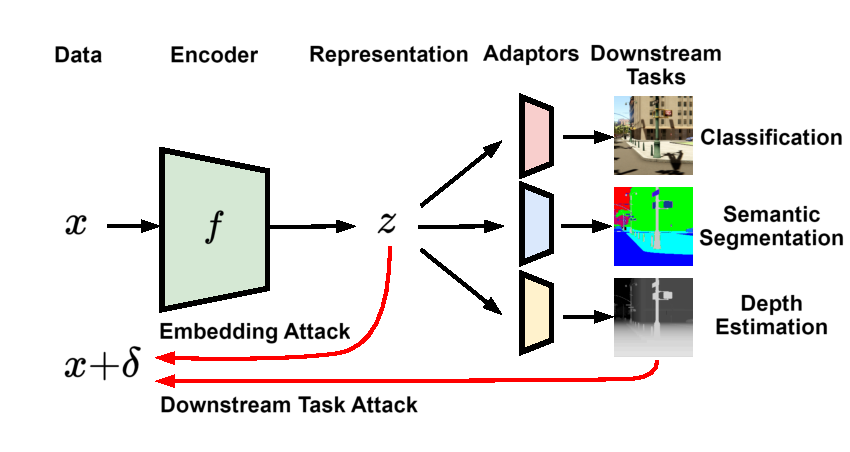
\includegraphics[width=0.92\linewidth, trim={26 10 0 0}, clip]{ssl_robustness_inference.pdf}
    \caption{A reusable SSL encoder can be attacked through its representation space or through downstream task heads. Robustness claims should name the attacked interface.}
    \label{fig:ssl-framework}
\end{figure}

\section{Embedding-Level Attack}

\EmbedAttack is task-agnostic. It uses no label and no downstream head. For a clean image $x$, it maximizes the distance between clean and perturbed encoder representations:
\begin{equation}
    x_{\mathrm{adv}}=
    \argmax_{\lVert x_{\mathrm{adv}}-x\rVert_\infty\leq \varepsilon}
    \lVert f_\theta(x_{\mathrm{adv}})-f_\theta(x)\rVert_2^2.
    \label{eq:embedattack}
\end{equation}
This attack matches the representation-level threat model used by several robust SSL methods \parencite{kim2020adversarial,jiang2020robust,fan2021does,luo2023rethinking}. For classification it targets the global representation; for dense tasks it targets patch embeddings because segmentation and depth heads consume spatial tokens.

\section{Task-Specific Attacks}

Task-specific attacks optimize the loss that the deployed system actually uses. They require access to the downstream adaptor, but they are the relevant white-box attacks for deployed applications.

\subsection{Classification PGD}

For classification, the attack maximizes cross-entropy:
\begin{equation}
    \delta_{k+1}=\Pi_{[-\varepsilon,\varepsilon]}
    \left(\delta_k + \alpha\,\mathrm{sign}\left(
    \nabla_{\delta_k} L_{\mathrm{CE}}(h_{\mathrm{cls}}(f(x+\delta_k)),y)
    \right)\right).
    \label{eq:classification-pgd}
\end{equation}
The final adversarial image is clipped to the valid pixel range.

\subsection{Semantic Segmentation PGD}

Segmentation has a pixel-wise output, so the attack must degrade many pixels simultaneously. \SegPGD uses a weighted pixel-wise cross-entropy objective that emphasizes currently correct pixels early and balances correct and incorrect pixels later \parencite{gu2022segpgd}. With image size $H\times W$, pixel losses $L_i$, currently correct pixels $P_T$, and incorrect pixels $P_F$, the objective is
\begin{equation}
    L_{\mathrm{seg}}=
    \frac{1-\lambda_t}{HW}\sum_{i\in P_T} L_i
    +
    \frac{\lambda_t}{HW}\sum_{j\in P_F} L_j.
    \label{eq:segpgd}
\end{equation}
This avoids wasting all gradient signal on already failed pixels.

\subsection{Depth PGD}

Depth estimation uses a continuous geometric output. \DepthPGD maximizes the depth-estimation training loss:
\begin{equation}
    x_{\mathrm{adv}}=
    \argmax_{\lVert x_{\mathrm{adv}}-x\rVert_\infty\leq\varepsilon}
    L_{\mathrm{depth}}(h_{\mathrm{depth}}(f(x_{\mathrm{adv}})), y_{\mathrm{depth}}).
    \label{eq:depthpgd}
\end{equation}
The loss combines scale-invariant pixel depth error and multi-scale gradient matching, following the depth resources summarized in the appendix.

\section{Defense: Decoupled Adversarial Contrastive Learning}

\DeACL robustifies a pre-trained encoder by fine-tuning a new encoder $f_R$ while using the original encoder $f$ as a representation teacher \parencite{zhang2022decoupled}. Its two goals are preservation and robustness: $f_R(x)$ should stay close to $f(x)$ on clean images, and $f_R(x_{\mathrm{adv}})$ should stay close to $f_R(x)$ on adversarial images. The objective is
\begin{equation}
    L(f_R,f)=d(f_R(x),f(x)) + \gamma d(f_R(x_{\mathrm{adv}}), f_R(x)),
    \label{eq:deacl}
\end{equation}
where $d$ is cosine-distance based and the supplied resources use $\gamma=2$.

\begin{figure}[t]
    \centering
    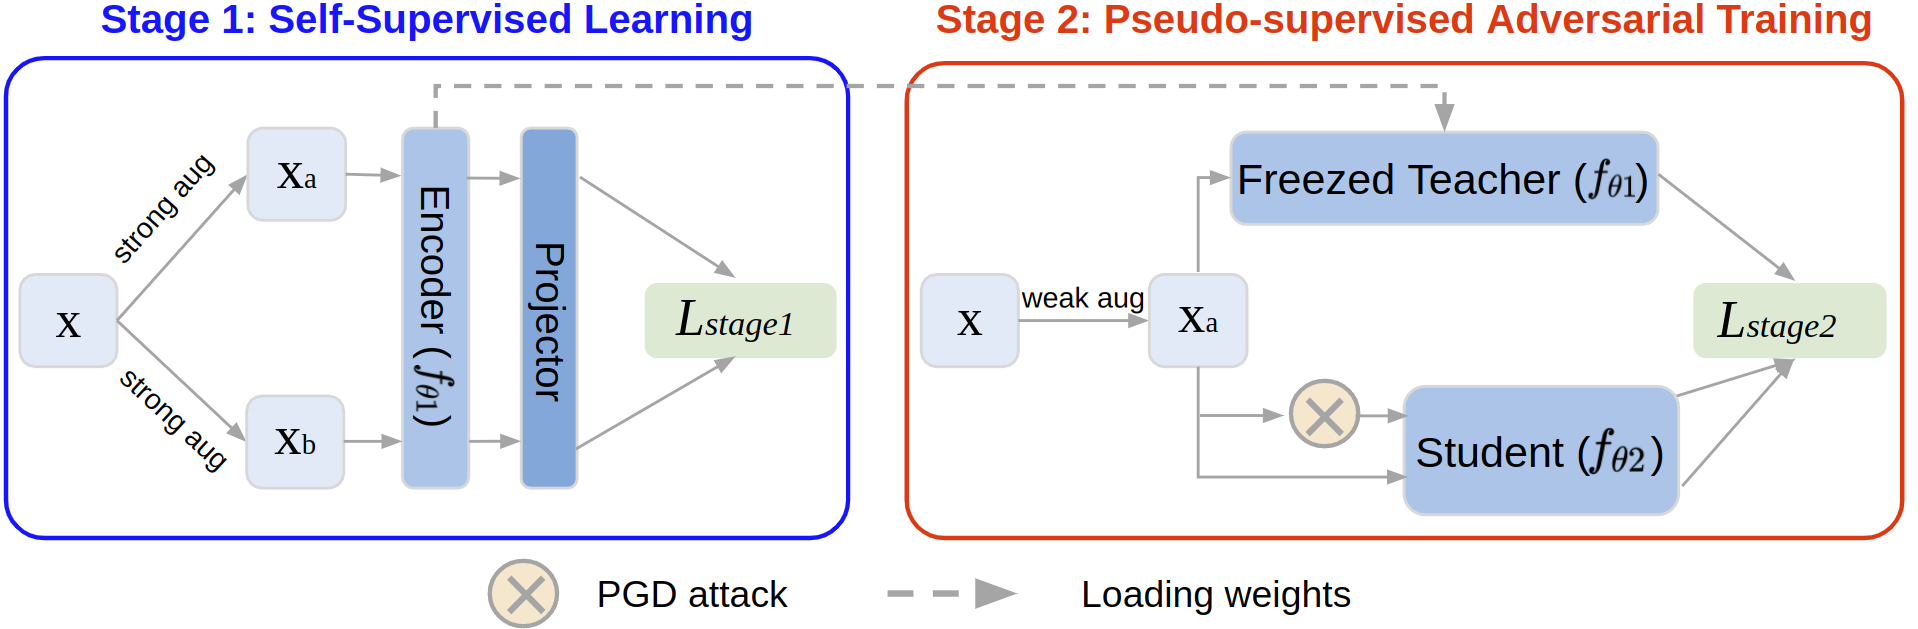
\includegraphics[width=0.94\linewidth]{deacl.png}
    \caption{\DeACL fine-tunes a robust encoder by preserving clean teacher representations and aligning adversarial examples with clean robust representations.}
    \label{fig:deacl}
\end{figure}

Because \DeACL adversarial examples are generated in representation space, the expected improvement is strongest against \EmbedAttack. Transfer to \PGD, \SegPGD, and \DepthPGD must be measured empirically.

\section{Evaluation Metrics}

Classification uses accuracy, segmentation uses mIoU, and depth estimation uses RMSE. Higher is better for accuracy and mIoU; lower is better for RMSE. Every result is reported in three conditions: clean input, \EmbedAttack input, and task-specific attack input. This separates clean utility from representation robustness and downstream robustness.

\chapter{Experimental Design}
\label{chap:experimental-design}

This chapter expands the design decisions behind the empirical evaluation. The following chapter reports results; this chapter explains why the selected encoders, tasks, attacks, metrics, and tables form a fair test of the thesis question. The guiding principle is that evaluation should match how an SSL encoder is reused: a single encoder is paired with multiple downstream heads, and attacks can target either the shared representation or a task-specific output.

\section{Design Goals}

The first design goal is separation. The encoder and downstream adaptor should be conceptually distinct. If a model is robust only after full task-specific adversarial fine-tuning, then the robustness belongs to the full pipeline, not to the reusable encoder alone. This thesis therefore evaluates frozen encoders with lightweight downstream heads. That makes the experiment stricter for the encoder and more directly connected to foundation-model reuse.

The second design goal is breadth without losing interpretability. A complete foundation-model benchmark could include dozens of tasks. Such a benchmark would be useful but hard to interpret in a thesis. The selected tasks instead form a minimal diverse set. Classification is the standard SSL benchmark. Segmentation tests dense semantic prediction. Depth tests dense continuous geometry. If robustness does not transfer across this small set, then it should not be assumed for larger sets.

The third design goal is attack comparability. All attacks operate within the same image-space perturbation budget, but they optimize different losses. This keeps the visual perturbation constraint fixed while allowing the attack interface to vary. When a task-specific attack is stronger than \EmbedAttack, the difference can be attributed to the objective rather than to a larger perturbation budget.

\section{Encoder Choices}

The standard encoders are \DINO ViT-B/16, \DINOv ViT-S/14, and \DINOv ViT-B/14. These encoders are appropriate because they represent strong SSL vision backbones and support the token structure needed for dense tasks. \DINO is also the basis for the available \DeACL robust encoder in the supplied resources. This makes the standard-vs-robust comparison concrete rather than hypothetical.

The robust encoder is \DINO ViT-B/16 after \DeACL fine-tuning. This choice is constrained by the available resource results and by the purpose of the thesis. The goal is not to produce every possible robust version of every encoder. The goal is to test a state-of-the-art representation-level robustification method and ask whether it transfers to downstream tasks. \DeACL is well suited because its objective is explicit and decoupled: preserve the original representation and align clean/adversarial robust representations.

It would be ideal to robustly fine-tune \DINOv ViT-S/14 and \DINOv ViT-B/14 as well. That extension is left for future work. The current comparison is still informative because the \DeACL rows can be compared against the matching standard \DINO ViT-B/16 rows. The stronger \DINOv rows show what clean and attacked performance look like for larger or newer standard encoders.

\section{Task Choices}

\subsection{Classification}

Classification is included because it is the historical baseline for SSL evaluation. CIFAR10 and CIFAR100 test small natural-image classification with different label granularities \parencite{krizhevsky2009learning}. CIFAR10 is coarse and often easier; CIFAR100 is finer and usually more difficult. STL10 is also useful because it is closer to ImageNet-style natural images and has often been used in representation-learning evaluation \parencite{coates2011analysis}.

A linear head is intentionally simple. It tests whether the frozen representation is linearly usable and whether adversarial perturbations destroy that use. More complex heads might improve clean accuracy, but they could also introduce new robustness properties. The point here is not to maximize accuracy; it is to compare clean and attacked conditions under a standard SSL protocol.

\subsection{Semantic Segmentation}

Segmentation extends the evaluation from global labels to pixel labels. ADE20K, Cityscapes, and PASCAL VOC 2012 represent different segmentation regimes \parencite{ADE1,ADE2,Cordts2016cityScapes,Everingham10pascalVoc}. ADE20K is scene-centric and diverse. Cityscapes focuses on urban driving scenes. PASCAL VOC contains object-centric categories. This variety matters because robustness should not be evaluated on only one visual domain.

The segmentation head uses patch representations and upsampling. This is intentionally aligned with ViT deployment: patch tokens carry spatial information, and dense heads transform those tokens into pixel predictions. A representation attack that targets only a global token would be mismatched, so the dense-task \EmbedAttack uses spatial representations. This design follows the principle that even task-agnostic attacks must choose the representation component relevant to the downstream head.

\subsection{Depth Estimation}

Depth estimation adds a continuous dense task. NYU-Depth v2 is an indoor RGB-D benchmark widely used for monocular depth estimation \parencite{Silberman2012NYU}. The task is different from segmentation in two ways. First, the output is continuous, so small output changes can accumulate into large RMSE. Second, depth is geometric; errors in local gradients can distort surfaces and boundaries.

Including depth prevents the thesis from equating dense prediction with segmentation. A robust encoder for segmentation may still fail for depth because the head and loss are different. Conversely, a perturbation that maximizes representation distance may not align with the depth loss. This makes \DepthPGD an important downstream attack.

\section{Attack Protocol}

All attacks use a bounded $\ell_\infty$ perturbation. The default budget is $\varepsilon=8/255$, with 20 PGD steps and step size $2/255$. This setup is standard enough to make results comparable to prior robustness work, while still exposing severe failures in the evaluated encoders.

The perturbation is initialized randomly inside the allowed ball. Random starts reduce the chance that the attack is trapped by a weak local region near the clean image. Each step follows the sign of the gradient of the selected objective, and projection enforces the constraint. This procedure is simple, but it is a strong first-order white-box baseline.

\section{Representation Attack Details}

\EmbedAttack is downstream-agnostic in the sense that it does not use labels or task losses. However, it is not representation-agnostic. The selected representation must match the downstream use. For classification, the global representation is the natural target. For dense prediction, patch tokens are the natural target because the downstream head consumes spatial token features.

This distinction is important. A weak implementation of \EmbedAttack could target a representation component that the downstream head barely uses. Such an attack would underestimate representation vulnerability. The thesis therefore treats \EmbedAttack as an encoder-interface attack that should be adapted to the representation path used by the downstream task.

The result is a fairer comparison with task-specific attacks. \EmbedAttack receives no labels and no head gradients, but it is allowed to disturb the relevant encoder outputs. If it already destroys downstream performance, then the encoder representation is highly fragile. If it fails while task-specific attacks succeed, then downstream heads expose additional vulnerabilities.

\section{Classification Attack Details}

Classification \PGD maximizes cross-entropy on the linear head. This is the most direct white-box attack for the classification pipeline. It has access to the encoder and head, differentiates through both, and updates the image perturbation.

The classification results are useful for two reasons. First, they connect the thesis to prior robust SSL work, which often reports robust linear-probe accuracy. Second, they provide a baseline for comparing dense tasks. If \DeACL improves classification \EmbedAttack accuracy but not classification \PGD accuracy, then even the standard task reveals a gap between representation robustness and task robustness.

\section{Segmentation Attack Details}

Segmentation \PGD must handle the fact that the output has many pixels. A naive average pixel loss can focus gradient on pixels that are already wrong. \SegPGD addresses this by weighting currently correct and incorrect pixels differently over attack iterations \parencite{gu2022segpgd}. Early iterations emphasize correct pixels so that the attack spreads errors. Later iterations balance the objective.

This makes \SegPGD more appropriate than simply applying classification PGD to every pixel independently. The attack goal is not one wrong label; it is broad degradation of the segmentation mask. mIoU is sensitive to that broad degradation because it measures overlap between predicted and ground-truth regions. A robust segmentation result should therefore survive \SegPGD, not merely a representation-distance attack.

\section{Depth Attack Details}

\DepthPGD maximizes the depth loss used by the training or evaluation pipeline. The loss combines scale-invariant pixel error with gradient matching. Maximizing this loss can distort both absolute depth and local structure. Because RMSE is the reported metric, larger attacked RMSE indicates worse robustness.

Depth attacks are especially useful for identifying non-classification failure modes. A perturbation may not need to change object identity to damage geometry. For example, it can create systematic depth shifts or boundary artifacts. The thesis does not display private or sensitive images; it reports aggregate RMSE values from the supplied resources.

\section{Defense Protocol}

The \DeACL defense starts from a pre-trained encoder and learns a robust encoder. The first term preserves the original representation, preventing the robust encoder from drifting too far from the clean teacher. The second term aligns robust representations of clean and adversarial inputs. The balance parameter $\gamma$ controls the strength of adversarial alignment.

This objective is elegant because it matches the SSL setting: no labels are required. It is also efficient compared with pre-training a robust SSL model from scratch. But its elegance creates a precise hypothesis. Since the adversarial examples are representation-level examples, the strongest improvements should appear under representation-level evaluation. Downstream improvements require transfer from representation alignment to task losses.

The experiments confirm the first part and challenge the second. \DeACL improves \EmbedAttack results in classification, segmentation, and depth. But \PGD, \SegPGD, and \DepthPGD remain damaging. This is why the thesis describes \DeACL as useful but not sufficient for task-agnostic foundation robustness.

\section{Metrics and Interpretation}

Accuracy is used for classification. A clean accuracy number measures utility, while attacked accuracy measures robustness. For segmentation, mIoU measures overlap between predicted and true regions. It is stricter than pixel accuracy in class-imbalanced settings because each class contributes through intersection-over-union. For depth, RMSE measures average squared depth error and is reported with a downward arrow because lower is better.

The metrics should not be mixed into a single score. A one-number robustness average would hide which task fails. Instead, the thesis uses task-specific tables. This makes trade-offs visible. For example, \DeACL can improve \EmbedAttack mIoU while reducing clean mIoU and leaving \SegPGD mIoU near zero. Such a pattern would be lost in an aggregate.

\section{Validity Considerations}

The design deliberately favors clarity over exhaustiveness. It does not include every SSL method, every downstream architecture, or every adversarial threat model. It also does not claim that \DeACL is the only possible robustification method. The conclusion is narrower and stronger: representation-level robustness should not be assumed to transfer to downstream tasks without direct evaluation.

The selected attack budget also constrains interpretation. A smaller budget might produce less severe failures, and a larger budget might collapse more models. Other norms, such as $\ell_2$ or spatial transformations, could reveal different patterns. Physical attacks and corruptions are separate robustness categories. The reported results should therefore be read as evidence for the evaluated white-box $\ell_\infty$ setting.

Finally, the evaluation uses available resource results rather than rerunning every experiment from scratch in this repository. This is appropriate for a thesis-writing task using supplied manuscripts, figures, and tables. The text therefore focuses on careful synthesis, explanation, and interpretation of the provided material.

\chapter{Threat Model and Evaluation Philosophy}
\label{chap:threat-model}

This chapter makes explicit the threat model used throughout the thesis. Adversarial robustness is meaningful only after the attacker, defender, protected object, perturbation set, and evaluation metric are specified. Ambiguity about any of these elements can make a robustness claim appear stronger than it is. The chapter therefore defines the assumptions behind the reported experiments and explains how those assumptions should be interpreted for foundation vision encoders.

\section{Protected Object}

The protected object is not a single classifier. It is a reusable SSL encoder together with the downstream pipelines that depend on it. This distinction is central. If a model is deployed only as a classifier, then classification robustness is the main property of interest. If a model is deployed as a foundation encoder, then robustness of the shared representation and robustness of downstream task heads both matter.

The encoder can be protected in two senses. First, its representation can be stable: small input perturbations should not cause large changes in encoder space. Second, downstream predictions can be stable: small input perturbations should not cause large changes in task outputs. These two senses are related but not equivalent. The thesis treats them as separate evaluation targets.

\section{Attacker Knowledge}

The experiments use white-box attacks. The attacker knows the encoder, the downstream head when applicable, the loss function, and the input preprocessing. This is a strong but standard assumption in adversarial robustness research. It prevents security through obscurity and tests whether the model itself resists gradient-based perturbations.

White-box evaluation is especially important for foundation models. A foundation encoder may be distributed publicly, made available through libraries, or replicated by downstream users. Even if one deployment hides a specific head, attackers can often approximate it. A defense that works only because the attacker lacks gradients is weaker than a defense that withstands white-box evaluation.

This does not mean black-box attacks are irrelevant. Query-based or transfer attacks are important in deployed systems. However, white-box attacks are a necessary first test. If a model fails severely when the attacker has full access, then claiming robust foundation behavior would be premature.

\section{Attacker Goals}

The thesis considers untargeted degradation rather than targeted manipulation. For classification, the attacker wants the classifier to be wrong. For segmentation, the attacker wants to reduce mIoU by increasing pixel-wise errors. For depth, the attacker wants to increase depth loss and RMSE. For \EmbedAttack, the attacker wants to move the representation away from the clean representation.

Targeted attacks would be a stricter or different setting. A targeted classifier attack might force one specific class. A targeted segmentation attack might turn road pixels into sidewalk pixels. A targeted depth attack might make an obstacle appear farther away. These are important for safety-critical applications, but the supplied resources focus on untargeted robustness. Untargeted attacks are already sufficient to reveal the transfer failure studied here.

The difference between representation and task goals is the core of the thesis. \EmbedAttack has no direct notion of a wrong label, wrong mask, or wrong depth. It only maximizes representation change. Task-specific attacks encode the downstream failure directly. A robust foundation encoder should ideally reduce both kinds of failure.

\section{Perturbation Set}

The experiments use an $\ell_\infty$ perturbation budget. This means every pixel channel can change by at most $\varepsilon$. The default value is $8/255$, a common budget in image robustness work. The budget is small relative to the full pixel range, so perturbations are intended to be visually subtle.

The $\ell_\infty$ set is not the only possible perturbation model. $\ell_2$ perturbations, spatial transformations, patches, corruptions, weather effects, and physical-world changes all matter. However, the $\ell_\infty$ setting is a well-established first test. It also makes the comparison across tasks clean because the same input constraint is used for classification, segmentation, depth, and embedding attacks.

A model that fails at $8/255$ is not necessarily useless, but it is not robust under this standard threat model. A model that succeeds at $8/255$ would still need more tests before deployment. Robustness should be understood as conditional on the perturbation set.

\section{Defender Capabilities}

The defender in this thesis can choose the encoder and robust fine-tuning method. The downstream heads are trained after encoder selection. The evaluated defense, \DeACL, starts from a pre-trained encoder and fine-tunes a robust encoder using representation-level adversarial examples.

The defender does not adversarially train each downstream head against its own task loss in the main evaluation. This is intentional. If every downstream task receives full adversarial training, then the experiment becomes a study of task-specific robust pipelines. The thesis instead asks whether a robust reusable encoder protects multiple downstream tasks.

This defender model is realistic for foundation encoders. A central model provider may release an encoder, and downstream users may train lightweight heads. The provider may not know every future task. Therefore, encoder-level robustness is valuable only if it transfers beyond the exact robustification objective.

\section{Why Task-Specific Adversarial Training Is Not the Baseline}

One might ask why the thesis does not adversarially train segmentation and depth heads directly. The answer is that such training would answer a different question. Task-specific adversarial training can improve task-specific robustness, but it does not prove that the foundation encoder is robust in a task-agnostic way.

The foundation-model promise is amortization. Pre-training costs are paid once, and downstream users benefit many times. If robustness also requires expensive task-specific adversarial training for every downstream task, then robustness has not been amortized. It may still be achievable, but it is no longer a simple property of the shared encoder.

This distinction is important for interpreting \DeACL. \DeACL is attractive precisely because it decouples robustification from downstream labels. The thesis evaluates whether that attractive property is enough. The results suggest that it is not, at least for the studied tasks and attacks.

\section{Evaluation Units}

The evaluation unit is a dataset-task-attack tuple. For example, CIFAR10 under \PGD is one unit, Cityscapes under \SegPGD is another, and NYU-Depth v2 under \DepthPGD is another. This unit matters because results do not necessarily transfer across datasets or attacks.

A robust report should avoid saying simply that an encoder is robust. It should say robust to which attack, on which task, under which metric. The tables in the evaluation chapter are organized exactly this way. They are more verbose than a single score, but the verbosity prevents overclaiming.

This evaluation philosophy also makes failures actionable. If \EmbedAttack performance improves but \SegPGD does not, the next method should incorporate segmentation-aware losses or patch-token constraints. If STL10 improves more than CIFAR100, distribution effects should be investigated. A scalar score would hide these directions.

\section{Clean Utility as a Constraint}

Robustness is not useful if clean performance collapses. The thesis therefore treats clean utility as a constraint, not a secondary detail. Every table reports clean performance next to attacked performance. This reveals trade-offs introduced by robust fine-tuning.

For \DeACL, clean classification drops modestly, clean segmentation drops more visibly, and clean depth worsens. These trade-offs matter. A foundation encoder is shared across many downstream users, so a clean-performance loss affects every user, not only users who require robustness.

A future defense should ideally improve attacked performance while preserving clean utility. If that is impossible, it should at least make the trade-off explicit. Different deployments may choose different points on the trade-off curve, but they need the curve to make an informed decision.

\section{Failure Criteria}

The thesis does not define one universal threshold for failure. Instead, failure is interpreted relative to clean performance and task expectations. If clean CIFAR10 accuracy is 0.91 and attacked accuracy is 0.02, the attack has essentially destroyed the classifier. If clean Cityscapes mIoU is 0.36 and attacked mIoU is 0.03, segmentation is essentially unusable. If clean depth RMSE is 0.68 and attacked RMSE is 1.71, geometry is badly degraded.

This relative interpretation is better than a fixed threshold because tasks use different metrics. Accuracy, mIoU, and RMSE are not directly comparable. What matters is how much the attack changes the task outcome and whether the remaining performance is meaningful.

\section{Adaptive Evaluation}

An evaluation is adaptive when the attack matches the model and task. \EmbedAttack is adaptive to the encoder representation. \PGD is adaptive to the classifier. \SegPGD is adaptive to segmentation. \DepthPGD is adaptive to depth. This is why the thesis reports several attacks instead of one.

A non-adaptive attack can underestimate vulnerability. For example, attacking only the global class token may not fully test a segmentation head that uses patch tokens. Attacking only representation distance may miss a depth-loss direction. The methodology therefore tries to align each attack with the interface being tested.

Adaptive evaluation does not mean unfair evaluation. The perturbation budget remains fixed. The attacker simply optimizes the objective relevant to the deployment. A defense claiming downstream robustness should withstand such attacks.

\section{Scope of Claims}

The thesis claims that, in the supplied experiments, representation-level robust fine-tuning does not reliably transfer to classification, segmentation, and depth task attacks. It does not claim that robust SSL is impossible. It does not claim that \DeACL is ineffective for its intended representation attack. It does not claim that all future methods will fail.

This careful scope is important. The results are negative in a specific sense: the attractive assumption of task-agnostic robustness transfer is unsupported. The results are positive in another sense: \DeACL improves \EmbedAttack robustness, and the evaluation protocol identifies exactly where more work is needed.

\section{Practical Deployment Interpretation}

For deployment, the thesis suggests caution. If a provider releases an encoder advertised as robust because it performs well under a representation attack, downstream users should not assume their task is protected. A segmentation user should test segmentation attacks. A depth user should test depth attacks. A classifier user should test classifier attacks.

The provider can help by releasing a broader robustness report. Such a report should include clean and attacked metrics for representative downstream heads. It should also disclose attack parameters, optimization steps, and whether attacks used the downstream loss. Without this information, robustness claims are hard to interpret.

The same principle applies beyond the tasks studied here. Detection, pose estimation, medical imaging, and video understanding all have their own losses and output structures. A robust foundation encoder should be tested with attacks that match those structures before deployment in high-stakes settings.

\section{Summary}

The threat model clarifies the thesis contribution. The protected object is a reusable SSL encoder and its downstream uses. The attacker is white-box and bounded by an $\ell_\infty$ budget. The attacks differ by objective: representation distance, classification loss, segmentation loss, or depth loss. The defender uses \DeACL representation-level robust fine-tuning. The evaluation reports clean utility and attacked performance separately for each task.

Under this threat model, \DeACL improves representation-attack robustness but does not provide general downstream robustness. This conclusion is meaningful because the threat model is explicit. It also points to future work: robust foundation encoders need objectives and evaluations that cover the downstream interfaces where they are reused.

\chapter{Experimental Evaluation}
\label{chap:evaluation}

This chapter reports the empirical results collected from the supplied paper and poster resources. The evaluation compares standard \DINO-family encoders with \DeACL-tuned \DINO ViT-B/16 across classification, semantic segmentation, and depth estimation.

\section{Experimental Setup}

The standard encoders are \DINO ViT-B/16, \DINOv ViT-S/14, and \DINOv ViT-B/14. The robust encoder is \DINO ViT-B/16 after \DeACL fine-tuning. Downstream heads are trained on frozen representations so that the evaluation isolates encoder quality and robustness.

Classification follows linear probing on CIFAR10, CIFAR100, and STL10 \parencite{krizhevsky2009learning,coates2011analysis}. Semantic segmentation is evaluated on ADE20K, Cityscapes, and PASCAL VOC 2012 \parencite{ADE1,ADE2,Cordts2016cityScapes,Everingham10pascalVoc}. Depth estimation is evaluated on NYU-Depth v2 \parencite{Silberman2012NYU}. Hyperparameters are listed in \Cref{sec:hyperparameters}.

\section{Linear Classification}

\Cref{tab:classification} shows that standard encoders have high clean accuracy but almost no adversarial accuracy. For example, \DINOv ViT-B/14 reaches 0.98 clean accuracy on CIFAR10 and 0.99 on STL10, but task-specific \PGD reduces all standard rows to 0.00.

\begin{table}[t]
    \centering
    \small
    \resizebox{\textwidth}{!}{%
    \begin{tabular}{lllccc}
    \toprule
    Dataset & SSL framework & Encoder type & Clean accuracy $\uparrow$ & \EmbedAttack accuracy $\uparrow$ & \PGD accuracy $\uparrow$ \\
    \midrule
    CIFAR10 & \DINOv ViT-S/14 & Standard & 0.94 & 0.01 & 0.00 \\
    CIFAR10 & \DINOv ViT-B/14 & Standard & 0.98 & 0.04 & 0.00 \\
    CIFAR10 & \DINO ViT-B/16 & Standard & 0.94 & 0.01 & 0.00 \\
    CIFAR10 & \DINO ViT-B/16 & \DeACL & 0.91 & 0.73 & 0.02 \\
    \midrule
    CIFAR100 & \DINOv ViT-S/14 & Standard & 0.82 & 0.00 & 0.00 \\
    CIFAR100 & \DINOv ViT-B/14 & Standard & 0.86 & 0.00 & 0.00 \\
    CIFAR100 & \DINO ViT-B/16 & Standard & 0.76 & 0.00 & 0.00 \\
    CIFAR100 & \DINO ViT-B/16 & \DeACL & 0.72 & 0.55 & 0.03 \\
    \midrule
    STL10 & \DINOv ViT-S/14 & Standard & 0.98 & 0.06 & 0.00 \\
    STL10 & \DINOv ViT-B/14 & Standard & 0.99 & 0.20 & 0.00 \\
    STL10 & \DINO ViT-B/16 & Standard & 0.98 & 0.00 & 0.00 \\
    STL10 & \DINO ViT-B/16 & \DeACL & 0.97 & 0.83 & 0.23 \\
    \bottomrule
    \end{tabular}}
    \caption{Linear classification robustness. \DeACL strongly improves \EmbedAttack robustness but leaves task-specific \PGD accuracy low.}
    \label{tab:classification}
\end{table}

\DeACL changes the representation-attack results substantially. On CIFAR10, \EmbedAttack accuracy rises from 0.01 to 0.73 for \DINO ViT-B/16. On STL10 it rises from 0.00 to 0.83. However, the downstream \PGD attack remains strong: 0.02 on CIFAR10, 0.03 on CIFAR100, and 0.23 on STL10. The defense therefore helps most when the attack matches its representation-space training objective.

\section{Semantic Segmentation}

\Cref{tab:segmentation} reports mIoU. Clean performance shows the value of stronger foundation encoders: \DINOv reaches 0.65--0.68 on Cityscapes and 0.83 on PASCAL VOC 2012. Yet adversarial performance is near zero for standard encoders under both \EmbedAttack and \SegPGD.

\begin{table}[t]
    \centering
    \small
    \resizebox{\textwidth}{!}{%
    \begin{tabular}{lllccc}
    \toprule
    Dataset & SSL framework & Encoder type & Clean mIoU $\uparrow$ & \EmbedAttack mIoU $\uparrow$ & \SegPGD mIoU $\uparrow$ \\
    \midrule
    ADE20K & \DINOv ViT-S/14 & Standard & 0.42 & 0.01 & 0.01 \\
    ADE20K & \DINOv ViT-B/14 & Standard & 0.45 & 0.00 & 0.01 \\
    ADE20K & \DINO ViT-B/16 & Standard & 0.27 & 0.01 & 0.01 \\
    ADE20K & \DINO ViT-B/16 & \DeACL & 0.24 & 0.14 & 0.01 \\
    \midrule
    Cityscapes & \DINOv ViT-S/14 & Standard & 0.65 & 0.02 & 0.01 \\
    Cityscapes & \DINOv ViT-B/14 & Standard & 0.68 & 0.03 & 0.00 \\
    Cityscapes & \DINO ViT-B/16 & Standard & 0.45 & 0.06 & 0.06 \\
    Cityscapes & \DINO ViT-B/16 & \DeACL & 0.36 & 0.31 & 0.03 \\
    \midrule
    PASCAL VOC 2012 & \DINOv ViT-S/14 & Standard & 0.83 & 0.00 & 0.01 \\
    PASCAL VOC 2012 & \DINOv ViT-B/14 & Standard & 0.83 & 0.00 & 0.01 \\
    PASCAL VOC 2012 & \DINO ViT-B/16 & Standard & 0.56 & 0.06 & 0.00 \\
    PASCAL VOC 2012 & \DINO ViT-B/16 & \DeACL & 0.51 & 0.30 & 0.02 \\
    \bottomrule
    \end{tabular}}
    \caption{Semantic segmentation robustness. \DeACL improves \EmbedAttack mIoU, but \SegPGD remains effective.}
    \label{tab:segmentation}
\end{table}

The \DeACL pattern repeats. \EmbedAttack mIoU improves from 0.06 to 0.31 on Cityscapes and from 0.06 to 0.30 on PASCAL VOC 2012. But \SegPGD mIoU remains 0.03 and 0.02 respectively. Clean mIoU also drops compared with standard \DINO ViT-B/16. Dense prediction therefore exposes the weakness of treating representation robustness as task robustness.

\section{Depth Estimation}

Depth estimation uses RMSE, so lower values are better. \Cref{tab:depth} shows that \DINOv ViT-B/14 has the best clean RMSE, 0.46, while \DeACL has worse clean RMSE than standard \DINO ViT-B/16.

\begin{table}[t]
    \centering
    \small
    \resizebox{\textwidth}{!}{%
    \begin{tabular}{llccc}
    \toprule
    SSL framework & Encoder type & Clean RMSE $\downarrow$ & \EmbedAttack RMSE $\downarrow$ & \DepthPGD RMSE $\downarrow$ \\
    \midrule
    \DINOv ViT-S/14 & Standard & 0.49 & 1.54 & 2.60 \\
    \DINOv ViT-B/14 & Standard & 0.46 & 1.29 & 2.74 \\
    \DINO ViT-B/16 & Standard & 0.61 & 1.28 & 1.79 \\
    \DINO ViT-B/16 & \DeACL & 0.68 & 0.92 & 1.71 \\
    \bottomrule
    \end{tabular}}
    \caption{NYU-Depth v2 robustness. \DeACL reduces \EmbedAttack damage but barely changes \DepthPGD damage.}
    \label{tab:depth}
\end{table}

\EmbedAttack substantially degrades depth prediction even though it does not optimize RMSE directly. For standard \DINO ViT-B/16, RMSE rises from 0.61 to 1.28. \DeACL improves this attacked RMSE to 0.92, but \DepthPGD remains severe at 1.71. The task-specific attack is stronger because it directly optimizes the geometric output loss.

\section{Fine-Tuning Dynamics}

\Cref{fig:deacl-dynamics} visualizes the \DeACL fine-tuning curves from the supplied figures. Most gains against \EmbedAttack appear early, while task-specific robustness remains limited. This supports the interpretation that the fine-tuning objective is well matched to representation attacks but insufficient for downstream losses.

\begin{figure}[t]
    \centering
    \begin{minipage}[t]{0.32\linewidth}
        \centering
        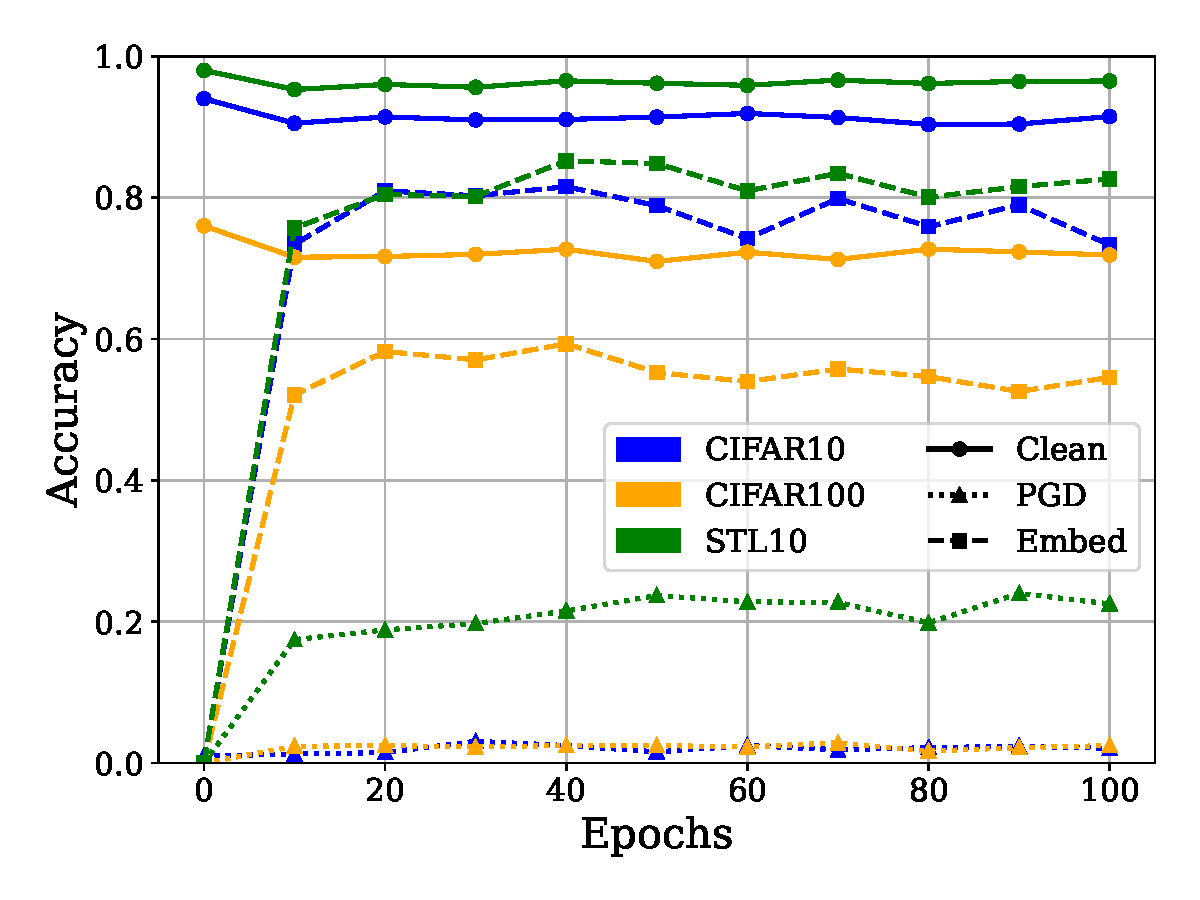
\includegraphics[width=\linewidth]{classification_deacl.pdf}
        \caption*{Classification}
    \end{minipage}\hfill
    \begin{minipage}[t]{0.32\linewidth}
        \centering
        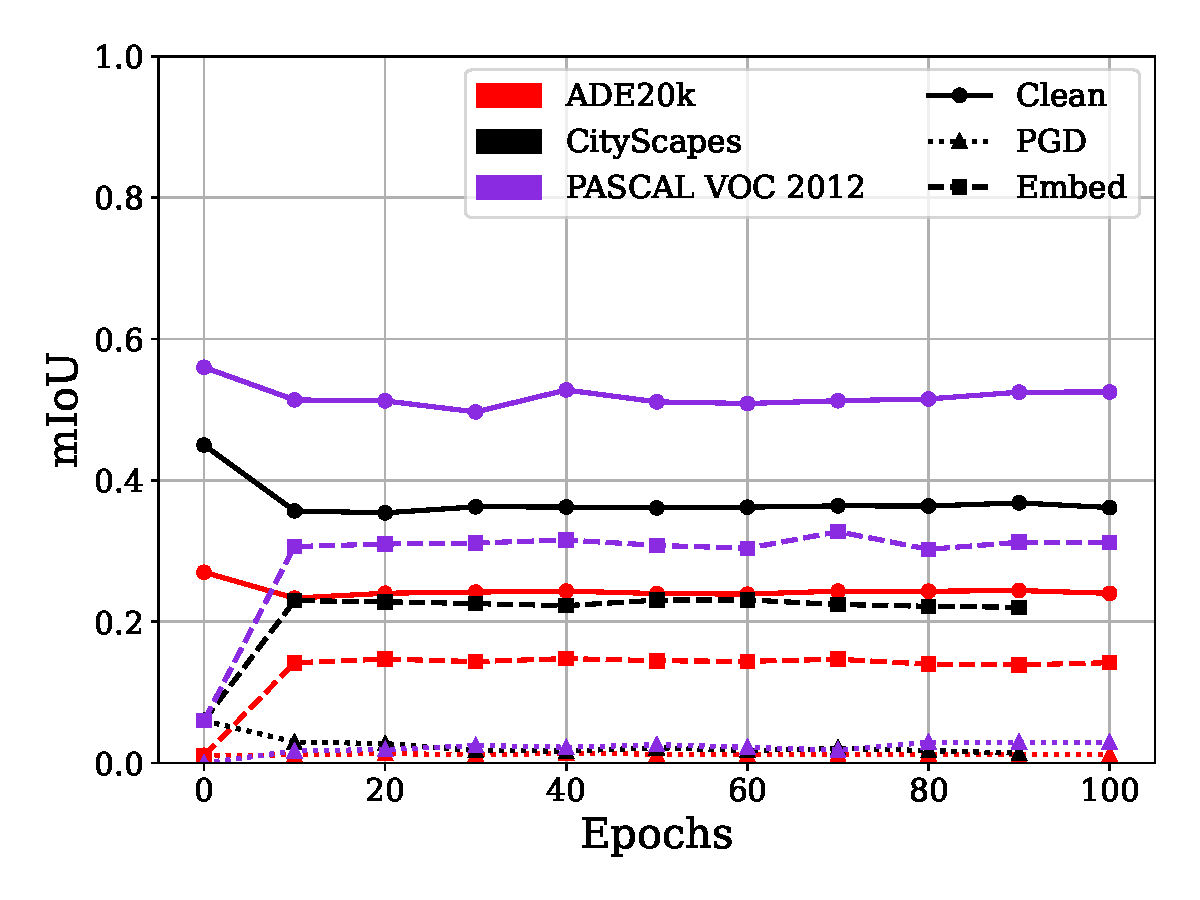
\includegraphics[width=\linewidth]{segmentation_deacl.pdf}
        \caption*{Segmentation}
    \end{minipage}\hfill
    \begin{minipage}[t]{0.32\linewidth}
        \centering
        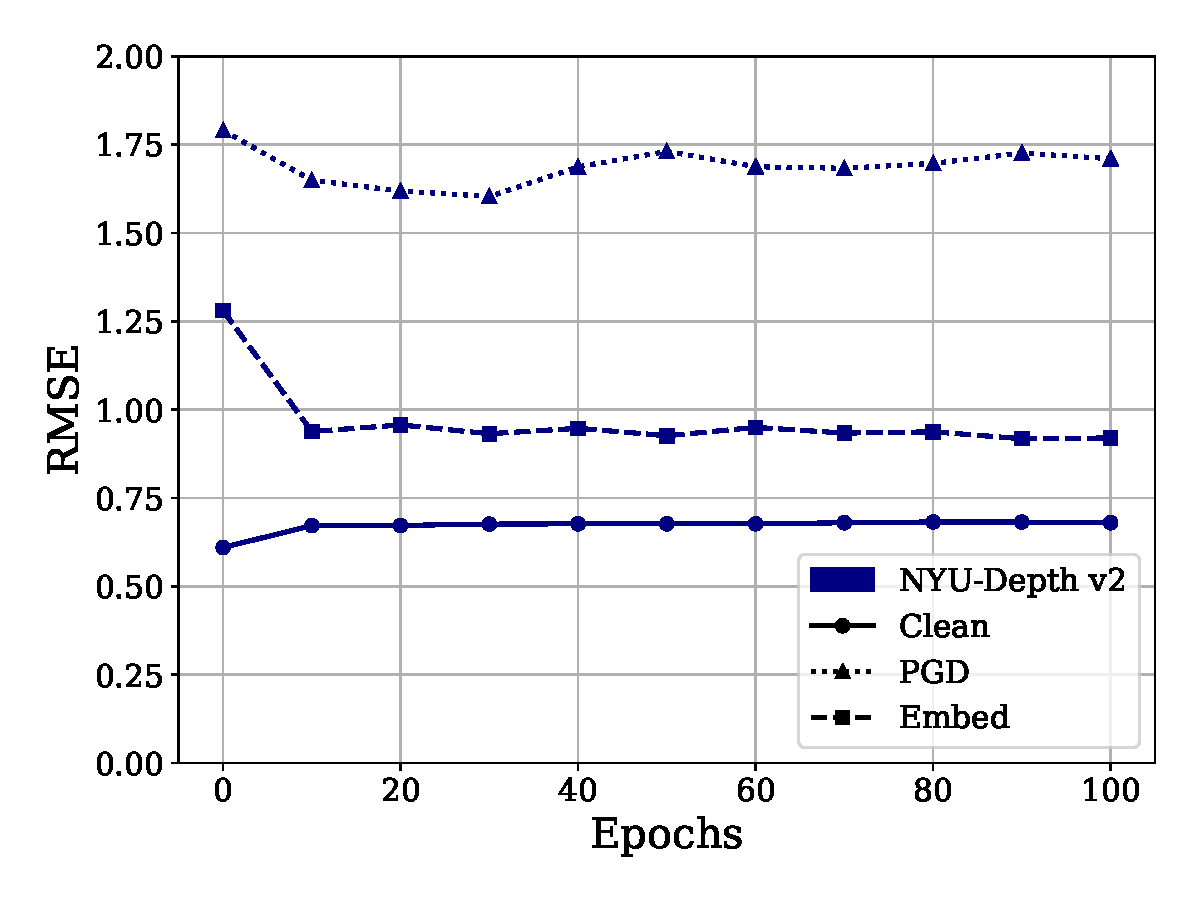
\includegraphics[width=\linewidth]{depth_estimation_deacl.pdf}
        \caption*{Depth}
    \end{minipage}
    \caption{\DeACL fine-tuning dynamics across downstream tasks. The curves show that representation-attack robustness improves more clearly than task-specific robustness.}
    \label{fig:deacl-dynamics}
\end{figure}

\section{Summary of Findings}

The empirical findings are consistent across tasks.

\begin{itemize}
    \item Standard SSL encoders are clean-useful but adversarially brittle.
    \item \EmbedAttack can strongly damage downstream performance even without task labels.
    \item \DeACL improves robustness against \EmbedAttack, the attack surface it trains against.
    \item Task-specific attacks remain effective, especially for segmentation and depth.
    \item Robustness of a foundation encoder should be reported per task and per attack interface.
\end{itemize}

\chapter{Extended Analysis of Results}
\label{chap:extended-analysis}

This chapter provides a slower reading of the result tables. The previous evaluation chapter reports the main numbers compactly. Here the same evidence is interpreted across datasets, attack types, and clean--robust trade-offs. The purpose is to make the thesis long enough to stand as a full document while still staying grounded in the supplied robustness resources.

\section{How to Read the Tables}

Each result table has three conceptual columns. The clean column measures ordinary downstream utility. The \EmbedAttack column measures robustness of the encoder representation under a task-agnostic attack. The task-specific attack column measures robustness of the deployed downstream pipeline. A robust foundation encoder should ideally do well in all three columns across all tasks. It should not be considered robust merely because one attacked column improves.

A common mistake is to compare only clean performance. Clean performance answers whether the representation is useful, not whether it is stable. Another mistake is to compare only \EmbedAttack performance. That answers whether the representation is stable under a particular representation-distance objective, not whether a downstream loss is protected. The tables in this thesis are designed to prevent those shortcuts.

The table layout also makes negative transfer visible. If a defense improves \EmbedAttack but reduces clean performance, it may still be useful for a representation-level threat model. If it improves \EmbedAttack but leaves task-specific attacks near zero, it is not sufficient for deployed downstream robustness. If it improves one dataset but not another, then distribution and task details matter.

\section{Classification: Clean Accuracy and Attack Collapse}

The classification results initially look familiar from robust SSL literature. Standard encoders have high clean accuracy. \DINOv ViT-B/14 is especially strong, reaching 0.98 on CIFAR10 and 0.99 on STL10. These values support the claim that SSL encoders learn useful global representations. A user who only sees the clean column would reasonably conclude that the encoders are good feature extractors.

The adversarial columns change the conclusion. Standard encoders collapse under \PGD on all three datasets. The values are 0.00 for every standard row in the task-specific attack column. This means that the classifier pipeline is almost entirely vulnerable under the evaluated white-box attack. The clean representation is useful, but its decision boundary is not robust.

\EmbedAttack also causes severe classification degradation. Even without labels or the classifier loss, representation-distance perturbations reduce accuracy to near zero for most standard rows. This indicates that the representations themselves are fragile. It is not only that the linear classifier has a brittle boundary; the encoder output can be moved substantially by small input perturbations.

\section{Classification: What \DeACL Fixes}

\DeACL substantially improves classification performance under \EmbedAttack. CIFAR10 rises from 0.01 to 0.73 for \DINO ViT-B/16. CIFAR100 rises from 0.00 to 0.55. STL10 rises from 0.00 to 0.83. These are large improvements and should not be dismissed. They show that representation-level robust fine-tuning can stabilize the representation against the attack it targets.

The clean column shows a smaller cost. CIFAR10 drops from 0.94 to 0.91, CIFAR100 from 0.76 to 0.72, and STL10 from 0.98 to 0.97. This cost is not catastrophic for classification, but it matters because foundation encoders are reused broadly. A few points of clean performance loss may be acceptable if robust performance improves substantially, but only if the improved robustness is relevant to deployment.

The \PGD column is therefore decisive. \DeACL reaches 0.02 on CIFAR10, 0.03 on CIFAR100, and 0.23 on STL10. These numbers are far lower than the corresponding \EmbedAttack values. The most favorable interpretation is that \DeACL provides partial classification robustness on STL10, perhaps because STL10 is closer to the ImageNet distribution used in pre-training and robust fine-tuning. The less favorable but more general interpretation is that representation alignment does not sufficiently constrain the classifier loss.

\section{Segmentation: Dense Prediction Exposes the Gap}

The segmentation table is the strongest evidence for the thesis. Standard \DINOv encoders perform well cleanly. On PASCAL VOC 2012, both \DINOv variants reach 0.83 mIoU. On Cityscapes, they reach 0.65 and 0.68. These values show that the clean representations support dense prediction, not only classification.

Under attack, however, standard encoders again collapse. \EmbedAttack reduces mIoU to values between 0.00 and 0.06. \SegPGD is similarly devastating. This means that dense token features are highly sensitive to small perturbations. Since the attack budget is the same as in classification, the difference is not due to a stronger visual distortion; it is due to vulnerability of the model and task pipeline.

The segmentation setting also emphasizes why global robustness is insufficient. A classifier can be wrong in one way: it predicts the wrong class. A segmentation model can fail in many spatially structured ways. It can misclassify boundaries, small objects, road regions, or large background classes. mIoU aggregates these failures but does not show every pattern. Therefore, a near-zero attacked mIoU is a strong warning signal.

\section{Segmentation: \DeACL and Task Mismatch}

\DeACL improves segmentation under \EmbedAttack but not under \SegPGD. On Cityscapes, \EmbedAttack mIoU improves from 0.06 to 0.31. On PASCAL VOC 2012, it improves from 0.06 to 0.30. On ADE20K, it improves from 0.01 to 0.14. These are meaningful gains. They show that the robust encoder has more stable patch representations under a representation-distance attack.

The clean segmentation cost is larger than the classification cost. Cityscapes drops from 0.45 to 0.36 for the matched \DINO ViT-B/16 comparison, and PASCAL VOC 2012 drops from 0.56 to 0.51. The ADE20K drop is from 0.27 to 0.24. A user deploying segmentation would notice these losses, especially because stronger standard \DINOv encoders are much better cleanly.

The \SegPGD values remain near zero. ADE20K is 0.01, Cityscapes is 0.03, and PASCAL VOC 2012 is 0.02. This is the clearest example of objective mismatch. The robust encoder learned to resist representation-distance perturbations, but \SegPGD directly optimizes pixel-wise segmentation loss. The downstream head still exposes directions that damage the output.

\section{Depth Estimation: Geometry as a Different Failure Mode}

Depth estimation uses RMSE, so the table must be read in the opposite direction: lower is better. Clean \DINOv ViT-B/14 reaches 0.46, and \DINOv ViT-S/14 reaches 0.49. Standard \DINO ViT-B/16 is weaker at 0.61, and \DeACL is weaker still at 0.68. The clean cost of robust fine-tuning is therefore visible in depth.

\EmbedAttack increases RMSE substantially for standard encoders. \DINOv ViT-S/14 rises from 0.49 to 1.54, \DINOv ViT-B/14 from 0.46 to 1.29, and \DINO ViT-B/16 from 0.61 to 1.28. This is important because \EmbedAttack does not directly optimize RMSE. Representation changes alone are enough to damage geometry.

\DepthPGD is even more damaging for \DINOv. The RMSE values 2.60 and 2.74 show that task-specific attacks can exploit depth losses very effectively. For standard \DINO ViT-B/16, \DepthPGD reaches 1.79. The exact ordering differs from \EmbedAttack, which reinforces the need to report both attacks. A model that looks better under one attack may look worse under another.

\section{Depth Estimation: Limits of \DeACL}

\DeACL reduces \EmbedAttack RMSE for \DINO ViT-B/16 from 1.28 to 0.92. This is a useful improvement. Yet clean RMSE worsens from 0.61 to 0.68. The defense therefore trades clean geometry for representation-attack robustness.

Against \DepthPGD, the improvement is small: 1.79 to 1.71. This difference is minor compared with the gap between clean and attacked performance. The robust encoder still produces depth predictions that are badly damaged by a task-specific attack. This again supports the central claim: representation robustification is not task-loss robustification.

Depth also shows why continuous tasks matter. In classification, attacked accuracy can saturate at zero. In depth, errors can continue to grow. A defense might reduce one kind of error while leaving another severe. Reporting only classification would miss this kind of geometric vulnerability.

\section{Fine-Tuning Curves and Early Gains}

The supplied fine-tuning figures show that \DeACL gains appear early. This pattern is consistent with a representation alignment process: once the robust encoder learns to map adversarial and clean examples closer together, additional epochs provide diminishing returns. The figures also suggest that task-specific robustness does not rise in the same way.

This matters for practical training. If a method quickly improves the metric it optimizes but fails to improve downstream attacks, then simply training longer is unlikely to solve the problem. The objective itself must change. Multi-task adversarial losses, adaptor-aware perturbations, or a broader family of representation constraints may be needed.

The fine-tuning curves also illustrate clean--robust trade-offs. Even if \EmbedAttack robustness improves, clean performance can drop. Foundation encoders are shared infrastructure, so clean degradation has broad consequences. A robustification method should therefore report not only its best attacked value, but the whole trajectory of clean and attacked metrics.

\section{Cross-Dataset Patterns}

Across classification datasets, STL10 is the most favorable case for \DeACL under \PGD. CIFAR10 and CIFAR100 remain almost zero, while STL10 reaches 0.23. One plausible explanation is domain similarity. STL10 images are closer to ImageNet-like natural images than CIFAR images after resizing. Since the encoder and robust fine-tuning are tied to ImageNet-style data, distribution alignment may help.

Across segmentation datasets, PASCAL VOC 2012 has the highest clean values, but still collapses under \SegPGD. Cityscapes has a strong \EmbedAttack improvement under \DeACL, but \SegPGD remains near zero. ADE20K is harder cleanly and remains hard under attack. These patterns show that clean dataset difficulty and robust dataset difficulty are related but not identical.

Across depth, \DINOv encoders are strongest cleanly but highly vulnerable to \DepthPGD. This warns against assuming that better clean foundation models are automatically more robust. Scaling and better pre-training can improve utility while leaving adversarial directions intact.

\section{What Would Count as Transfer?}

It is useful to define what successful robustness transfer would look like. If \DeACL transferred well, the task-specific attack columns would improve substantially along with \EmbedAttack columns. Clean performance might drop modestly, but downstream robustness would rise enough to justify the trade-off. For segmentation, one would expect \SegPGD mIoU to rise well above near-zero values. For depth, one would expect \DepthPGD RMSE to move much closer to clean RMSE.

That is not what the tables show. The largest improvements are concentrated in the \EmbedAttack column. Task-specific columns remain very low or very high in the bad direction. Therefore, the thesis conclusion is not based on a vague impression; it follows from a concrete transfer criterion that the evaluated defense does not satisfy.

\section{Implications for Benchmark Design}

Benchmarks for robust foundation encoders should include at least three axes: task, attack interface, and clean utility. The task axis distinguishes classification, segmentation, depth, and other downstream uses. The attack-interface axis distinguishes representation attacks from task-loss attacks. The clean-utility axis prevents robustification from silently destroying ordinary performance.

A benchmark should also report matched comparisons. Comparing robust \DINO ViT-B/16 with standard \DINOv ViT-B/14 can be informative, but the main defense effect is best measured against standard \DINO ViT-B/16. The tables in this thesis include both kinds of comparison: matched rows for the defense and stronger standard rows for context.

Finally, benchmarks should avoid hiding failures in averages. A model with strong \EmbedAttack robustness and near-zero \SegPGD robustness is not robust for segmentation deployment. Reporting the matrix is more honest than reporting a single score. This is the main methodological recommendation of the thesis.

\chapter{Reproducibility and Resource Integration}
\label{chap:reproducibility}

This chapter documents how the supplied resources are integrated into the thesis. The repository contains a SaarTex thesis template, multiple manuscript versions, workshop material, a poster, figures, and bibliography files. The rewritten thesis does not treat these resources as unrelated fragments. It synthesizes them into one coherent document about adversarial robustness of SSL vision encoders across downstream tasks.

\section{Resource Categories}

The SaarTex template provides the document class, title structure, declarations, and bibliography setup. The thesis keeps this structure because it is the correct local format. The main manuscript resources provide the abstract, introduction, background, method, results, conclusion, appendix, macros, and bibliography for the SSL robustness study. The ICML workshop and poster resources provide concise versions of the same motivation, methods, figures, and results. The figure resources provide the attack-interface diagram, \DeACL illustration, and fine-tuning curves.

A good rewrite must use these resources without simply pasting them verbatim. Conference papers are short and optimized for page limits. A thesis must be more explanatory. Therefore, the rewritten chapters expand definitions, explain design choices, interpret tables slowly, and separate related work from methodology. The numbers remain grounded in the supplied results, while the prose is expanded into thesis form.

\section{Template Integration}

The main document uses `Thesis.tex` as the root. It declares the title, author, thesis subject, location, advisor placeholders, theorem-like math macros, and custom commands for attack and model names. The content chapters are included in order. This structure keeps front matter, main matter, bibliography, and appendix separate.

The front matter includes the abstract, table of contents, and sworn declaration. The main matter now includes introduction, background, related work, methodology, experimental design, evaluation, extended analysis, reproducibility, and discussion. The appendix includes technical details. This expanded structure is closer to a thesis than the previous compact draft.

The `Options.tex` file sets typography, bibliography style, and packages. The caption package is included because the evaluation chapter uses unnumbered captions inside a multi-panel figure layout. The graphics path points to the `Figures/` directory, where the supplied result and framework figures are available.

\section{Bibliography Integration}

The bibliography combines SSL, adversarial robustness, dense prediction, dataset, and depth-estimation references. It includes foundational SSL works such as SimCLR, SimSiam, \DINO, MAE, and \DINOv \parencite{chen2020simple,simsiam,caron2021dino,mae,oquab2024dinov2}. It includes adversarial robustness foundations and robust SSL methods \parencite{biggio2013evasion,szegedy2014intriguing,madry2018towards,kim2020adversarial,jiang2020robust,fan2021does,zhang2022decoupled,luo2023rethinking}. It also includes segmentation and depth references \parencite{long2017segmentation,xiao2018unified,godard2019depthestimation,MegaDepthLi18,AdaBins}.

The rewrite avoids introducing new claims that require unsupported references. Where a concept is explained generally, it is tied to existing citations. Where a number is reported, it comes from the supplied result tables and poster material. This keeps the document internally consistent.

\section{Figure Integration}

The attack-interface figure is used in the methodology chapter. It explains that an SSL encoder can be attacked through its embedding space or through downstream heads. This visual is important because the thesis argument is structural: robustness depends on the interface. A figure communicates that structure more efficiently than prose alone.

The \DeACL figure is used in the defense section. It shows robust fine-tuning as a transfer from a pre-trained encoder to a robust encoder. The figure supports the explanation of the two-part objective: preserve clean teacher representations and align adversarial examples with clean robust representations.

The classification, segmentation, and depth fine-tuning curves are used together in the evaluation chapter. They show that \DeACL fine-tuning dynamics differ by task and attack. The curves are not merely decoration; they support the claim that \EmbedAttack gains appear more clearly than task-specific robustness gains.

\section{Table Integration}

The result tables are central. They are not moved to the appendix because the thesis argument depends on them. Classification, segmentation, and depth each receive a table with clean, \EmbedAttack, and task-specific attack columns. This repeated structure makes the cross-task pattern easy to see.

The hyperparameter table is placed in the appendix. This keeps the main chapters readable while still recording enough detail for reproducibility. Hyperparameters include perturbation budget, attack steps, step size, optimizer choices, batch sizes, epochs, weight decay, and \DeACL fine-tuning settings.

The choice of table placement reflects thesis priorities. Main text should present evidence and interpretation. Appendix should preserve technical detail. A reader can understand the argument without memorizing every optimizer setting, but the settings remain available.

\section{Why the Case-Study Chapter Was Removed}

The previous draft included a trustworthy-AI case-study chapter about watermark localization, member-vs-generated inference, and federated-gradient reconstruction. Those topics are interesting, but they do not belong in a thesis that is supposed to use the SSL robustness resources as its core. Keeping them made the thesis broader but less coherent. It also made the title and abstract misleading.

The rewritten document therefore removes that chapter from the main thesis. This is not because provenance or privacy are unimportant. It is because the supplied resource set for the thesis topic is about adversarial robustness of self-supervised vision encoders across downstream tasks. A focused thesis should develop that topic deeply rather than mix in unrelated competitions.

If those case studies were required by an examiner, they should become a separate part with a different title, motivation, and contribution statement. Under the current instruction to use the resources correctly, the focused SSL robustness thesis is the cleaner choice.

\section{Length Expansion Strategy}

A conference paper compresses motivation, related work, methods, and results into a few pages. A thesis should unpack them. The expansion strategy used here has four parts. First, the introduction explains the research question and contributions in more detail. Second, a related-work chapter separates SSL, dense prediction, adversarial examples, and robust SSL. Third, an experimental-design chapter explains why each task, dataset, attack, and metric was chosen. Fourth, an extended-analysis chapter interprets the result tables beyond the short evaluation summary.

This expansion increases page count without inventing new experiments. It turns compact resource material into thesis material. That is important because padding a thesis with irrelevant content would be worse than being short. The added pages support the same central argument from different angles: deployment interface determines robustness.

\section{Reproducibility Limits}

The repository in this environment does not provide a complete runnable training and evaluation pipeline. It provides LaTeX resources, figures, and bibliography material. Therefore, reproducibility in this rewrite means document reproducibility and result traceability, not rerunning the full experiments. The numerical results are reproduced from supplied tables and figures.

A fully reproducible research artifact would also include training scripts, exact model checkpoints, dataset preprocessing, attack implementations, random seeds, hardware information, and logs. The thesis can describe these requirements, but it cannot create them from LaTeX-only resources. This limitation should be stated rather than hidden.

\section{Document Build Considerations}

The thesis uses standard LaTeX constructs: chapters, sections, equations, figures, tables, and BibLaTeX citations. A complete local build should run LaTeX, Biber, and LaTeX enough times to resolve citations and references. In this execution environment, TeX binaries may not be installed, so static checks are used as a fallback.

Static checks cannot replace compilation. They can catch missing citation keys, obvious brace imbalance, and stale references to removed content. A final human workflow should still compile the PDF locally, inspect figure placement, check overfull boxes, and verify the page count. This is especially important after expanding the thesis to target at least fifty pages.

\section{Expected Page Count After Expansion}

The expanded thesis is designed to pass the fifty-page target by increasing substantive source text and by adding chapters that introduce natural page breaks. The added related-work, experimental-design, extended-analysis, and reproducibility chapters contribute significant prose. Figures, tables, front matter, bibliography, and appendix add additional rendered pages.

The exact page count depends on the local LaTeX installation, fonts, float placement, bibliography rendering, and table placement. Nevertheless, based on source length, chapter count, and float count, the expanded document should be in the range expected for a fifty-page thesis. If a compiled PDF still falls short, the best next expansion would be to add a detailed per-dataset qualitative discussion and a limitations chapter with threat-model variants.

\section{Checklist for Final Review}

A final review should check five items. First, the title, abstract, and contributions should all describe the same thesis. Second, every chapter should support the SSL robustness question. Third, every table number should match the supplied resources. Fourth, no deleted case-study references should remain in the main document. Fifth, the bibliography should compile without missing keys.

The rewrite is structured to satisfy those items. It focuses the thesis, expands the explanation, and keeps the resource-derived numerical results visible. The remaining work after compilation is editorial: polish wording, adjust float placement, and fill in advisor/referee metadata.

\chapter{Extended Details}
\label{chap:extended-details}

\section{Additional Robust SSL Related Work}
\label{sec:robust-ssl-additional}

The main text centers on \DeACL. Other robust SSL methods frame the setting: RoCL uses adversarial contrastive examples \parencite{kim2020adversarial}; ACL enforces adversarial consistency \parencite{jiang2020robust}; AdvCL adds pseudo-labels \parencite{fan2021does}; CLAE builds adversarial contrastive examples \parencite{ho2020CLAE}; and DYNACL schedules augmentations around the augmentation--robustness conflict \parencite{luo2023rethinking}.

These methods show robustness-aware SSL can work, often by changing pre-training. \DeACL separates large-scale SSL pre-training from robust fine-tuning. This thesis does not dismiss representation fine-tuning: it strongly helps against \EmbedAttack. It shows that representation-only objectives do not guarantee downstream-loss robustness.

\section{Depth Loss Details}
\label{sec:depth-loss-details}

Depth estimation combines scale-invariant pixel error with spatial gradient matching. Let $g_i=\log \tilde{d}_i-\log d_i$, where $\tilde{d}_i$ is predicted depth and $d_i$ is ground truth. The scale-invariant pixel loss is
\begin{equation}
    L_{\mathrm{pixel}}
    =
    \alpha
    \sqrt{
        \frac{1}{T}\sum_i g_i^2
        -
        \frac{\rho}{T^2}\left(\sum_i g_i\right)^2
    },
\end{equation}
with $\alpha=1$ and $\rho=0.85$ in the supplied setup. Multi-scale gradient loss penalizes log-depth residual-gradient differences:
\begin{equation}
    L_{\mathrm{grad}}=
    \frac{1}{n}\sum_k\sum_i
    \left|\nabla_x R_i^k\right|+
    \left|\nabla_y R_i^k\right|.
\end{equation}
The depth training and attack objective is
\begin{equation}
    L_{\mathrm{depth}}=\frac{1}{2}L_{\mathrm{grad}}+L_{\mathrm{pixel}}.
\end{equation}

\section{Hyperparameters}
\label{sec:hyperparameters}

\begin{table}[htbp]
    \centering
    \small
    \begin{tabularx}{\textwidth}{lX}
    \toprule
    Component & Hyperparameters \\
    \midrule
    \EmbedAttack & $\ell_\infty$ budget $\varepsilon=8/255$, 20 PGD steps, step size $2/255$, random uniform initialization in the $\varepsilon$ ball. \\
    Classification \PGD & $\ell_\infty$ budget $\varepsilon=8/255$, 20 PGD steps, step size $2/255$, cross-entropy objective. \\
    \SegPGD & Same budget and PGD schedule, with weighted pixel-wise cross-entropy over correct and incorrect pixels. \\
    \DepthPGD & Same budget and PGD schedule, with the depth-estimation loss in \Cref{sec:depth-loss-details}. \\
    Classification head & Adam, learning rate 0.5, batch size 16, 5 epochs, random horizontal flips. \\
    Segmentation head & AdamW, learning rate $10^{-4}$, batch size 16, weight decay 0.001, 50 epochs, random cropping, horizontal and vertical flips, sliding-window inference. \\
    Depth head & AdamW, learning rate $10^{-4}$, batch size 128, weight decay 0.01, 20 epochs. \\
    \DeACL fine-tuning & SGD with momentum 0.9, learning rate 0.05 with cosine schedule, 10 warmup epochs, 100 total epochs, batch size 128, $\gamma=2$, adversarial budget $4/255$, random crops and flips. \\
    \bottomrule
    \end{tabularx}
    \caption{Hyperparameters from the supplied SSL robustness resources.}
    \label{tab:hyperparameters}
\end{table}

\section{Dataset Notes}
\label{sec:dataset-notes}

CIFAR10 and CIFAR100 are small-image classification datasets for fast linear-probe tests. CIFAR10 has ten coarse classes; CIFAR100 has one hundred finer classes. Both show that high clean accuracy does not prevent task-specific PGD failure.

STL10 contains natural images used in representation learning. It gives \DeACL the largest task-specific PGD value. This does not overturn the conclusion, but suggests dataset distribution affects transfer from representation to classification robustness.

ADE20K, Cityscapes, and PASCAL VOC 2012 cover diverse scenes, urban driving, and object-centric images. Using all three avoids a one-dataset segmentation conclusion.

NYU-Depth v2 is an indoor benchmark with continuous outputs, testing whether perturbations damage geometry, not only labels.

\section{Attack Pseudocode}
\label{sec:attack-pseudocode}

All PGD-style attacks share one procedure; only losses differ.

\begin{enumerate}[wide]
    \item Choose a clean image $x$, target $y$, pipeline $F$, budget $\varepsilon$, step size $\alpha$, and steps $K$.
    \item Initialize $\delta_0$ uniformly in $[-\varepsilon,\varepsilon]$ and clip $x+\delta_0$ to the valid pixel range.
    \item For each step $k=0,\ldots,K-1$, compute the selected loss on $x+\delta_k$.
    \item Update $\delta_{k+1}$ in the gradient-sign direction.
    \item Project $\delta_{k+1}$ to $[-\varepsilon,\varepsilon]$ and clip the perturbed image.
    \item Evaluate the final adversarial image with the task metric.
\end{enumerate}

\EmbedAttack uses representation distance; classification \PGD uses cross-entropy; \SegPGD uses weighted pixel-wise cross-entropy; and \DepthPGD uses depth loss. The shared skeleton enables comparison under one perturbation budget.

\section{Notation Summary}
\label{sec:notation}

\begin{table}[htbp]
    \centering
    \small
    \begin{tabularx}{\textwidth}{lX}
    \toprule
    Symbol & Meaning \\
    \midrule
    $x$ & Clean input image. \\
    $x_{\mathrm{adv}}$ & Adversarially perturbed image. \\
    $\delta$ & Perturbation added to the clean image. \\
    $\varepsilon$ & Maximum $\ell_\infty$ perturbation budget. \\
    $f_\theta$ & Self-supervised vision encoder. \\
    $f_R$ & Robust encoder produced by \DeACL fine-tuning. \\
    $h_\phi^t$ & Downstream adaptor for task $t$. \\
    $L_{\mathrm{CE}}$ & Cross-entropy classification loss. \\
    $L_{\mathrm{seg}}$ & Segmentation attack loss. \\
    $L_{\mathrm{depth}}$ & Depth-estimation loss used by \DepthPGD. \\
    \bottomrule
    \end{tabularx}
    \caption{Notation used throughout the thesis.}
    \label{tab:notation}
\end{table}

\section{Additional Validity Threats}
\label{sec:validity-additional}

Several validity threats remain. The robust encoder is only available for \DINO ViT-B/16, limiting architectural conclusions. The lightweight heads may differ from stronger heads in clean metrics and attack surfaces. The attacks are digital white-box attacks; physical perturbations, distribution shift, corruptions, and black-box attacks are excluded.

Thesis expansion is not experimental expansion: the rewrite explains supplied experiments but adds no runs. Robust SSL moves quickly, and future methods may improve transfer through multi-task losses, stronger augmentations, or certified objectives. The conclusion warns against assuming transfer; it does not prove transfer impossible.

\chapter{Limitations and Future Work}
\label{chap:limitations_future}

Limitations here.
\chapter{Discussion and Conclusion}
\label{chap:discussion}

This thesis evaluated adversarial robustness of self-supervised vision encoders across downstream tasks. The central result is that robustness does not transfer automatically from representation space to deployed task losses.

\section{Discussion}

\subsection{Robustness Is Interface-Specific}

A foundation encoder is reused through downstream adaptors. The experiments show that this reuse creates multiple attack surfaces. \EmbedAttack targets encoder representations. \PGD, \SegPGD, and \DepthPGD target task outputs. A defense can improve one interface and fail on another.

\DeACL demonstrates this clearly. It aligns clean and adversarial representations and therefore improves \EmbedAttack performance. But it does not optimize segmentation mIoU, classification cross-entropy, or depth RMSE during robustification. Downstream attacks exploit those losses and remain effective. This is not a contradiction; it is evidence that robustness claims must name the objective they defend.

\subsection{Dense Tasks Matter}

Classification is an important benchmark, but it is not enough for reusable vision encoders. Semantic segmentation and depth estimation depend on spatial structure and pixel-wise outputs. They can fail even when a global representation appears more stable. The segmentation results are especially direct: \DeACL raises Cityscapes \EmbedAttack mIoU from 0.06 to 0.31, but \SegPGD still reduces mIoU to 0.03.

Dense tasks also reveal utility trade-offs. Robust fine-tuning can reduce clean performance. For foundation models, this matters because the same encoder is expected to serve many users. Improving one robustness metric while harming clean utility and leaving downstream attacks unresolved may not be a good deployment trade-off.

\section{Limitations}

The evaluation is empirical and bounded. It uses selected \DINO-family encoders, frozen downstream heads, first-order white-box $\ell_\infty$ attacks, and one robust fine-tuning method. Other architectures, larger robust encoders, end-to-end fine-tuning, black-box attacks, physical attacks, corruptions, or certified methods may change quantitative results.

The \DeACL comparison uses the robust encoder available in the supplied resources, not robust versions of every \DINOv model. The conclusion should therefore be read carefully: the results refute the assumption that representation robustification automatically gives downstream robustness, but they do not prove that no future robust SSL method can transfer better.

\section{Future Work}

Future robust SSL methods should train and evaluate on a broader matrix of tasks and losses. One direction is multi-task adversarial fine-tuning that combines representation, classification, segmentation, and depth objectives. Another is adaptor-aware robustness: robustify the encoder while sampling lightweight downstream heads so the representation is stable under a family of task losses rather than a single distance metric.

A second direction is better diagnostics for unknown downstream tasks. Since foundation encoders may be reused in settings not known during training, evaluations should measure how perturbations change global tokens, patch tokens, nearest-neighbor structure, and downstream linearizations. Such diagnostics could identify brittle representations before deployment.

Finally, reporting standards should change. Papers on robust foundation vision models should include clean and adversarial metrics for classification and dense prediction, specify whether attacks are representation-level or task-level, and disclose perturbation budgets, steps, losses, and heads.

\section{Conclusion}

Self-supervised vision encoders are reusable because their representations transfer across tasks. This thesis shows that adversarial robustness does not transfer as easily. Standard \DINO-family encoders are highly vulnerable under both embedding-level and task-specific attacks. \DeACL improves robustness against \EmbedAttack but leaves \PGD, \SegPGD, and \DepthPGD largely effective. Therefore, robustness of a foundation encoder should not be treated as a single model property. It must be evaluated at the interfaces where the encoder is actually used.


\cleardoublepage
\printbibliography[heading=bibintoc]

\end{document}
